\documentclass[,]{book}
\usepackage{lmodern}
\usepackage{amssymb,amsmath}
\usepackage{ifxetex,ifluatex}
\usepackage{fixltx2e} % provides \textsubscript
\ifnum 0\ifxetex 1\fi\ifluatex 1\fi=0 % if pdftex
  \usepackage[T1]{fontenc}
  \usepackage[utf8]{inputenc}
\else % if luatex or xelatex
  \ifxetex
    \usepackage{mathspec}
  \else
    \usepackage{fontspec}
  \fi
  \defaultfontfeatures{Ligatures=TeX,Scale=MatchLowercase}
\fi
% use upquote if available, for straight quotes in verbatim environments
\IfFileExists{upquote.sty}{\usepackage{upquote}}{}
% use microtype if available
\IfFileExists{microtype.sty}{%
\usepackage{microtype}
\UseMicrotypeSet[protrusion]{basicmath} % disable protrusion for tt fonts
}{}
\usepackage{hyperref}
\hypersetup{unicode=true,
            pdftitle={Graphically Based Data Analysis Using Flexplot},
            pdfkeywords={flexplot, statistical assumptions, NHST, replication crisis,
visualization, exploratory data analysis, graphical data analysis},
            pdfborder={0 0 0},
            breaklinks=true}
\urlstyle{same}  % don't use monospace font for urls
\ifnum 0\ifxetex 1\fi\ifluatex 1\fi=0 % if pdftex
  \usepackage[shorthands=off,main=]{babel}
\else
  \usepackage{polyglossia}
  \setmainlanguage[]{}
\fi
\usepackage{color}
\usepackage{fancyvrb}
\newcommand{\VerbBar}{|}
\newcommand{\VERB}{\Verb[commandchars=\\\{\}]}
\DefineVerbatimEnvironment{Highlighting}{Verbatim}{commandchars=\\\{\}}
% Add ',fontsize=\small' for more characters per line
\usepackage{framed}
\definecolor{shadecolor}{RGB}{248,248,248}
\newenvironment{Shaded}{\begin{snugshade}}{\end{snugshade}}
\newcommand{\KeywordTok}[1]{\textcolor[rgb]{0.13,0.29,0.53}{\textbf{#1}}}
\newcommand{\DataTypeTok}[1]{\textcolor[rgb]{0.13,0.29,0.53}{#1}}
\newcommand{\DecValTok}[1]{\textcolor[rgb]{0.00,0.00,0.81}{#1}}
\newcommand{\BaseNTok}[1]{\textcolor[rgb]{0.00,0.00,0.81}{#1}}
\newcommand{\FloatTok}[1]{\textcolor[rgb]{0.00,0.00,0.81}{#1}}
\newcommand{\ConstantTok}[1]{\textcolor[rgb]{0.00,0.00,0.00}{#1}}
\newcommand{\CharTok}[1]{\textcolor[rgb]{0.31,0.60,0.02}{#1}}
\newcommand{\SpecialCharTok}[1]{\textcolor[rgb]{0.00,0.00,0.00}{#1}}
\newcommand{\StringTok}[1]{\textcolor[rgb]{0.31,0.60,0.02}{#1}}
\newcommand{\VerbatimStringTok}[1]{\textcolor[rgb]{0.31,0.60,0.02}{#1}}
\newcommand{\SpecialStringTok}[1]{\textcolor[rgb]{0.31,0.60,0.02}{#1}}
\newcommand{\ImportTok}[1]{#1}
\newcommand{\CommentTok}[1]{\textcolor[rgb]{0.56,0.35,0.01}{\textit{#1}}}
\newcommand{\DocumentationTok}[1]{\textcolor[rgb]{0.56,0.35,0.01}{\textbf{\textit{#1}}}}
\newcommand{\AnnotationTok}[1]{\textcolor[rgb]{0.56,0.35,0.01}{\textbf{\textit{#1}}}}
\newcommand{\CommentVarTok}[1]{\textcolor[rgb]{0.56,0.35,0.01}{\textbf{\textit{#1}}}}
\newcommand{\OtherTok}[1]{\textcolor[rgb]{0.56,0.35,0.01}{#1}}
\newcommand{\FunctionTok}[1]{\textcolor[rgb]{0.00,0.00,0.00}{#1}}
\newcommand{\VariableTok}[1]{\textcolor[rgb]{0.00,0.00,0.00}{#1}}
\newcommand{\ControlFlowTok}[1]{\textcolor[rgb]{0.13,0.29,0.53}{\textbf{#1}}}
\newcommand{\OperatorTok}[1]{\textcolor[rgb]{0.81,0.36,0.00}{\textbf{#1}}}
\newcommand{\BuiltInTok}[1]{#1}
\newcommand{\ExtensionTok}[1]{#1}
\newcommand{\PreprocessorTok}[1]{\textcolor[rgb]{0.56,0.35,0.01}{\textit{#1}}}
\newcommand{\AttributeTok}[1]{\textcolor[rgb]{0.77,0.63,0.00}{#1}}
\newcommand{\RegionMarkerTok}[1]{#1}
\newcommand{\InformationTok}[1]{\textcolor[rgb]{0.56,0.35,0.01}{\textbf{\textit{#1}}}}
\newcommand{\WarningTok}[1]{\textcolor[rgb]{0.56,0.35,0.01}{\textbf{\textit{#1}}}}
\newcommand{\AlertTok}[1]{\textcolor[rgb]{0.94,0.16,0.16}{#1}}
\newcommand{\ErrorTok}[1]{\textcolor[rgb]{0.64,0.00,0.00}{\textbf{#1}}}
\newcommand{\NormalTok}[1]{#1}
\usepackage{longtable,booktabs}
\usepackage{graphicx,grffile}
\makeatletter
\def\maxwidth{\ifdim\Gin@nat@width>\linewidth\linewidth\else\Gin@nat@width\fi}
\def\maxheight{\ifdim\Gin@nat@height>\textheight\textheight\else\Gin@nat@height\fi}
\makeatother
% Scale images if necessary, so that they will not overflow the page
% margins by default, and it is still possible to overwrite the defaults
% using explicit options in \includegraphics[width, height, ...]{}
\setkeys{Gin}{width=\maxwidth,height=\maxheight,keepaspectratio}
\IfFileExists{parskip.sty}{%
\usepackage{parskip}
}{% else
\setlength{\parindent}{0pt}
\setlength{\parskip}{6pt plus 2pt minus 1pt}
}
\setlength{\emergencystretch}{3em}  % prevent overfull lines
\providecommand{\tightlist}{%
  \setlength{\itemsep}{0pt}\setlength{\parskip}{0pt}}
\setcounter{secnumdepth}{5}
% Redefines (sub)paragraphs to behave more like sections
\ifx\paragraph\undefined\else
\let\oldparagraph\paragraph
\renewcommand{\paragraph}[1]{\oldparagraph{#1}\mbox{}}
\fi
\ifx\subparagraph\undefined\else
\let\oldsubparagraph\subparagraph
\renewcommand{\subparagraph}[1]{\oldsubparagraph{#1}\mbox{}}
\fi

%%% Use protect on footnotes to avoid problems with footnotes in titles
\let\rmarkdownfootnote\footnote%
\def\footnote{\protect\rmarkdownfootnote}

%%% Change title format to be more compact
\usepackage{titling}

% Create subtitle command for use in maketitle
\providecommand{\subtitle}[1]{
  \posttitle{
    \begin{center}\large#1\end{center}
    }
}

\setlength{\droptitle}{-2em}

  \title{Graphically Based Data Analysis Using Flexplot}
    \pretitle{\vspace{\droptitle}\centering\huge}
  \posttitle{\par}
    \author{true}
    \preauthor{\centering\large\emph}
  \postauthor{\par}
      \predate{\centering\large\emph}
  \postdate{\par}
    \date{r Sys.Date()}

\usepackage[english]{babel}

\begin{document}
\maketitle

{
\setcounter{tocdepth}{1}
\tableofcontents
}
\chapter*{Introduction}\label{introduction}
\addcontentsline{toc}{chapter}{Introduction}

In light of the recent ``replication crisis'' (Pashler and Wagenmakers
2012; Open Science Collaboration 2015), researchers are becoming
increasingly concerned with the validity of science (Baker 2016). As
such, many are pushing for greater transparency and reproducibility
(Nelson, Simmons, and Simonsohn 2018; Nosek et al. 2018). One way to
accomplish greater transparency is through abudant use of data
visualizations (Tay et al. 2016), particularly when data are presented
in their raw form.

In addition to answering the call for greater transparency, graphics
offer several additional advantages. First, they improve communication
between the scientific community and the public. Lay people can
understand relatively sophisticated statistical procedures when that
information is presented graphically (Correll 2015). Additionally,
graphics highlight problems with models that are masked by traditional
statistical procedures, such as nonlinearity, outliers,
heteroscedasticity, etc. As such, graphics serve as an important
diagnostic check. Finally, graphics improve encoding. Consider the image
displayed in Figure \ref{fig:smiley}, taken from Correll (2015). The
table on the left presents the same information as the one on the right,
though the encoding of the information on the right is much easier
because that information is conveyed \emph{visually.}

\begin{figure}

{\centering 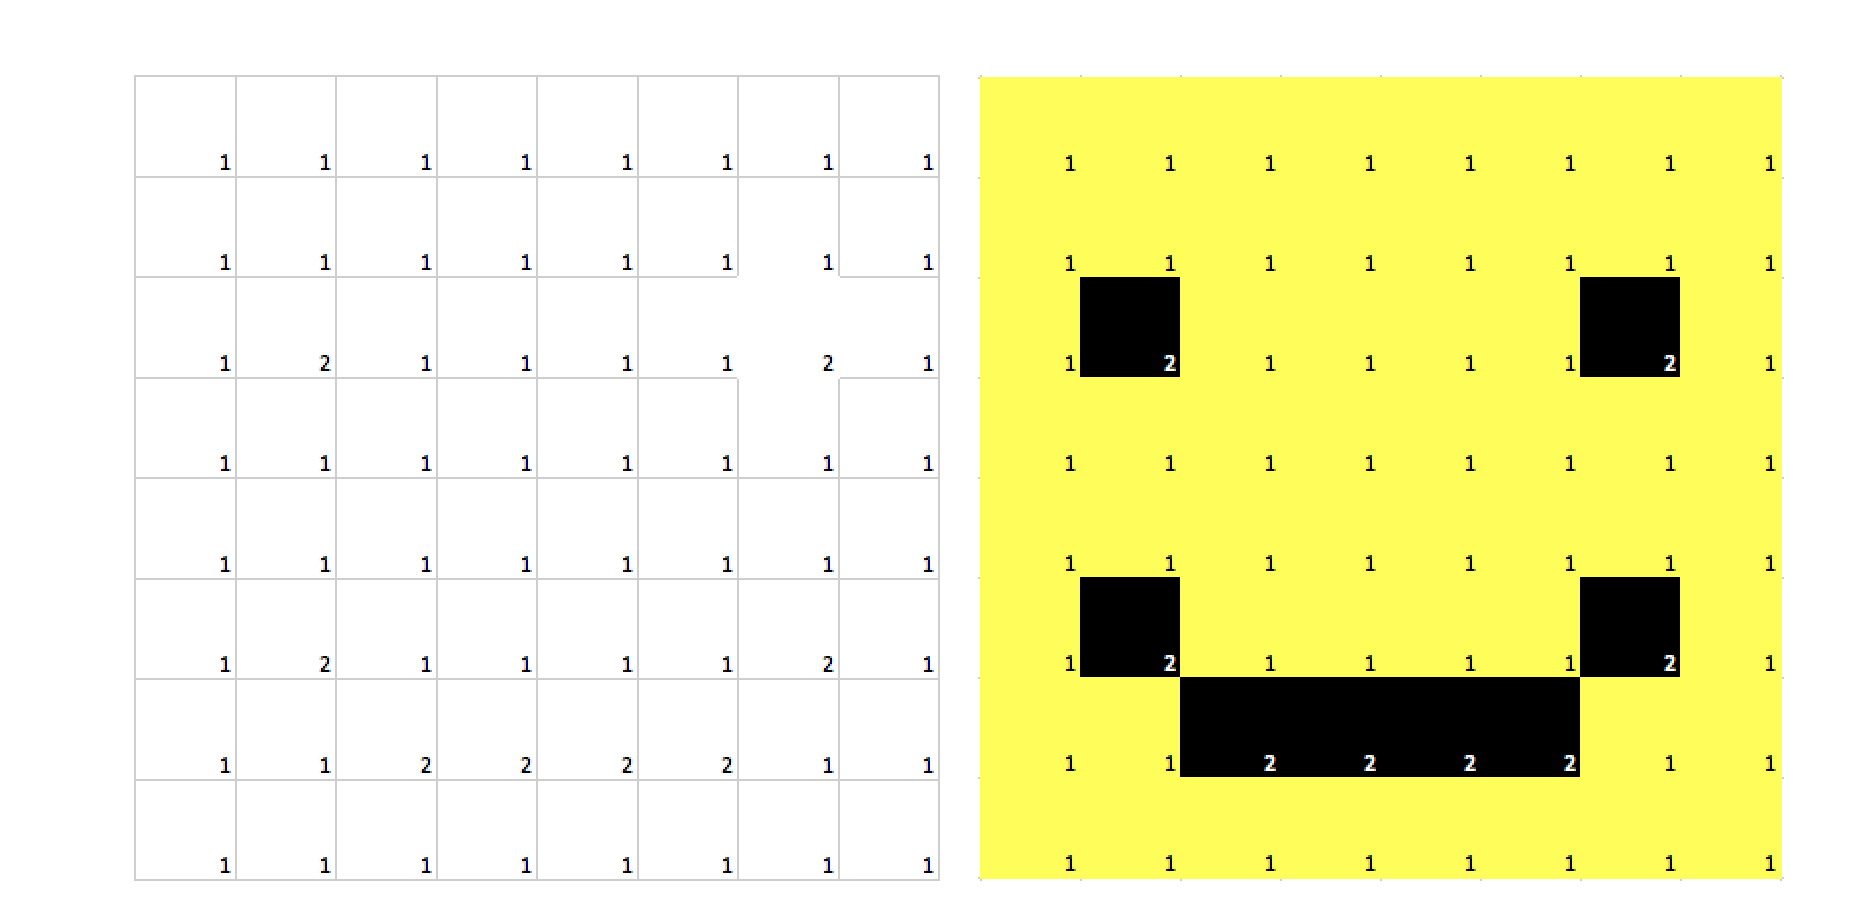
\includegraphics[width=26in]{images/smiley} 

}

\caption{A table of numbers on the left, and a color-coded table on the right, where the 2's have been highlighted in yellow. With the color, a pattern emerges that was not easy to see without the graphic. Figure used with permission from @Correll2015a}\label{fig:smiley}
\end{figure}

While visualizations have many advantages, they can also be used to
mislead, sometimes intentionally, and sometimes not intentionally. For
example, when means/standard errors are presented as barcharts, people
tend to judge values below the mean (i.e., within the confines of the
bar) as far more likely than values above the mean, even when the
underlying distribution is symmetric (Correll 2015). Unfortunately,
aesthetics are often conflated with informativeness, and people often
convince themselves they are learning something important from poor
graphics (Padilla et al. 2015). To further complicate matters, the
default images in most point-and-click statistical software violate
important visualization heuristics (Fife 2019). For example, in SPSS it
is impossible (as far as I know) to produce standard error plots that
display raw data (jittered or otherwise). Also, with standard error
plots, the axes are scaled to the means, not the range of the actual
data, which visually inflates the size of the effect. In addition,
producing some types of graphics (e.g., Skew-Location plots) require
more effort than many are willing to perform (the user must model the
data, export the residuals, jitter the residuals, then produce a
scatterplot).

Flexplot was designed to address these limitations. Flexplot was
developed using empirically-derived heurstics that maximize perceptual
understanding, while minimizing perceptual biases. Also, the graphics
produced are simple to generate and permit analysts to quickly shift
between statistical modeling and graphical interpretation.

\chapter*{Guiding Philosophy of
Flexplot}\label{guiding-philosophy-of-flexplot}
\addcontentsline{toc}{chapter}{Guiding Philosophy of Flexplot}

The design of Flexplot is based on the following principles:

\emph{1. Minimize obstacles to producing graphics.} The easier it is to
produce graphics, the more likely graphics will be used, and the more
resources the researcher will have available to interpret the data.
Technology companies like Apple and Google spend millions of dollars
attempting to make the interaction between humans and technology as
seamless as possible. One-click purchasing, voice-activated personal
assistants like Siri, movies-on-demand, and audible app notifications
are all tricks companies use to remove obstacles to using their
technology. Likewise, if producing a graphic is as simple (or simpler)
than performing a statistical analysis, they too will become heavily
utilized (and, dare I say, addictive?). Furthermore, the less effort
required to produce graphics, the more resources available to invest in
\emph{interpreting} graphics. To make producing graphics as simple as
possible, Flexplot makes many of the plotting decisions in the
background, such as choosing between types of graphics (e.g., histograms
versus bar charts) and how those graphics are displayed.

\emph{2. Design graphics that leverage human strenths and mitigate human
biases.} Successful technology capitalizes on human strengths. A mobile
phone, for example, leverages humanity's advanced finger tactile
sensitivity and dexterity. A phone designed to be used by one's foot
would be a very poor choice indeed. Likewise, a computer that sends
olefactory information might work well for a dog, but not a human.
Graphics technology ought to be designed with the same principles in
mind. Unfortunately, standard statistical analyses do not capitalize on
human strengths. It takes a great deal of training to understand even
basic statistics, and even then results are frequently misinterpreted.
To overcome this limitation, some of the tools within Flexplot create
visual representation of the statistical models. These representations
highlight uncertainty, reveal whether chosen models are appropriate, and
improve encoding of statistical information.

\chapter*{A New Grammar of Graphics}\label{a-new-grammar-of-graphics}
\addcontentsline{toc}{chapter}{A New Grammar of Graphics}

Hadley Wickham, the author of \texttt{ggplot2}, developed a ``layered''
grammar of graphics (Wickham 2010). Wickham's grammar allows a great
deal flexibility in the design of graphics. However, this flexibility
comes at cost. Very often the grammar necessary to produce a graphic
requires a great deal of coding to produce. For example, consider the
code to create jittered mean plots:

\begin{Shaded}
\begin{Highlighting}[]
\NormalTok{plot =}\StringTok{ }\KeywordTok{ggplot}\NormalTok{(}\DataTypeTok{data=}\NormalTok{exercise_data, }\KeywordTok{aes}\NormalTok{(}\DataTypeTok{x=}\NormalTok{therapy.type, }\DataTypeTok{y=}\NormalTok{weight.loss)) }\OperatorTok{+}
\StringTok{  }\KeywordTok{geom_jitter}\NormalTok{(}\DataTypeTok{amount=}\NormalTok{.}\DecValTok{2}\NormalTok{, }\DataTypeTok{alpha=}\NormalTok{.}\DecValTok{4}\NormalTok{) }\OperatorTok{+}
\StringTok{  }\KeywordTok{stat_summary}\NormalTok{(}\DataTypeTok{fun.y=}\StringTok{'mean'}\NormalTok{, }\DataTypeTok{geom=}\StringTok{'point'}\NormalTok{, }
               \DataTypeTok{size=}\DecValTok{3}\NormalTok{, }\DataTypeTok{position=}\KeywordTok{position_dodge}\NormalTok{(}\DataTypeTok{width=}\NormalTok{.}\DecValTok{2}\NormalTok{)) }\OperatorTok{+}
\StringTok{  }\KeywordTok{stat_summary}\NormalTok{(}\DataTypeTok{geom=}\StringTok{'errorbar'}\NormalTok{, }\DataTypeTok{fun.ymin =} \ControlFlowTok{function}\NormalTok{(z)\{}\KeywordTok{mean}\NormalTok{(z)}\OperatorTok{-}\FloatTok{1.96}\OperatorTok{*}\KeywordTok{sd}\NormalTok{(z)\}, }
               \DataTypeTok{fun.ymax=}\ControlFlowTok{function}\NormalTok{(z) \{}\KeywordTok{mean}\NormalTok{(z)}\OperatorTok{+}\FloatTok{1.96}\OperatorTok{*}\KeywordTok{sd}\NormalTok{(z)\}, }
               \DataTypeTok{size=}\FloatTok{1.25}\NormalTok{, }\DataTypeTok{width=}\NormalTok{.}\DecValTok{2}\NormalTok{, }\DataTypeTok{position=}\KeywordTok{position_dodge}\NormalTok{(}\DataTypeTok{width=}\NormalTok{.}\DecValTok{2}\NormalTok{)) }
\end{Highlighting}
\end{Shaded}

As noted earlier, the more difficult it is to produce a graphic, the
more likely it is someone will simply not use it. A similar graphic can
be produced with only one line of code using the \texttt{flexplot()}
function:

\begin{Shaded}
\begin{Highlighting}[]
\NormalTok{plot =}\StringTok{ }\KeywordTok{flexplot}\NormalTok{(weight.loss}\OperatorTok{~}\NormalTok{therapy.type, }\DataTypeTok{data=}\NormalTok{exercise_data)}
\end{Highlighting}
\end{Shaded}

Naturally, this simplicity comes at a cost; Flexplot is more limited
than ggplot2. However, Flexplot will cover the majority of graphics
analysts will use for statistical modeling. However, in the end,
graphics produced through Flexplot are still \texttt{ggplot2} objects.
As such, they can be edited and/or layered for further customization.

Flexplot's grammar is based on the general linear model (GLM). Recall
that most statistical procedures are subsumed within the GLM, which is
essentially regression. For example, a t-test is simply a regression
where the intercept is the mean of the referent group (e.g., the control
group) and the slope is simply the difference between the treatment and
control groups. The base R function \texttt{lm} utilizes GLMs to do
various sorts of modeling, and all this is accomplished using a simple
equation (e.g., \texttt{y\textasciitilde{}x1\ +\ x2}). Likewise,
Flexplot adopts the same convention, utilizing a similar equation to
produce graphics. Figure xxx shows an illustration that shows what
components of a Flexplot equation produce what elements of a grahpic.
The first variable in the equation (\(X1\)) specifies which variable is
displayed on the \(X\) axis. The second variable (\(X2\)) is displayed
as different colors/symbols/lines. The third and fourth elements are
shown as row and column panels, respectively. By following the grammar
of a GLM, there is perfect alignment between statistical modeling and
visualization, with a few notable exceptions. Most obviously, a GLM
equation (e.g.,
\texttt{plot(y\textasciitilde{}x1\ +\ x2\ +\ x3,\ data=data)}) does not
have any vertical pipes (\texttt{\textbar{}}) as \texttt{flexplot()}
does. This is necessary in \texttt{flexplot()} to allow more specificity
in paneling. Additionally, with GLMs, one must explicitly specify
interaction and polynomial terms. This isn't necessary with
\texttt{flexplot()}; the raw data are displayed exactly as they are and
if interactions are present, the visual will show it.

The base \texttt{plot()} function in R follows similar conventions to
Flexplot (i.e., users can specify an equation, such as
\texttt{plot(y\textasciitilde{}x)}), though \texttt{flexplot()} is more
intelligent in its choices of displays. Also, \texttt{plot()} only
allows the user to visualize one variable at a time. Another function,
\texttt{coplot()}, allows some multivariate visualizations, yet it is
limited in the types of data allowed and, like \texttt{plot()} isn't
flexible in the types of visualization decisions it makes. The Flexplot
package, on the other hand, offers great flexibility and automates much
of the decision-making.

In the following section, I will demonstrate how decisions are made in
Flexplot. I begin by showing how to produce univariate graphics, then
bivariate graphics, then multivariate graphics. I will then follow that
up with various functions and techniques for combining visuals with
models, then conclude with a brief summary.

\chapter*{Univariate Graphics}\label{univariate-graphics}
\addcontentsline{toc}{chapter}{Univariate Graphics}

In \texttt{lm()}, one can model an ``intercept only'' model, using the
code \texttt{lm(y\textasciitilde{}1)}. This is equivalent to estimating
the mean of \(y\). Flexplot follows a similar convention with
visualizing univariate distributions. However, the type of graphic
displayed depends on the type of variable inputted into the function.
For example, in the code below, notice that \texttt{flexplot()}
recognizes whether the variable is categorical or numeric, and plots
accordingly.

\begin{Shaded}
\begin{Highlighting}[]
\KeywordTok{require}\NormalTok{(flexplot)}
\KeywordTok{data}\NormalTok{(exercise_data)}
\NormalTok{a =}\StringTok{ }\KeywordTok{flexplot}\NormalTok{(weight.loss}\OperatorTok{~}\DecValTok{1}\NormalTok{, }\DataTypeTok{data=}\NormalTok{exercise_data)}
\NormalTok{b =}\StringTok{ }\KeywordTok{flexplot}\NormalTok{(gender}\OperatorTok{~}\DecValTok{1}\NormalTok{, }\DataTypeTok{data=}\NormalTok{exercise_data)}
\NormalTok{cowplot}\OperatorTok{::}\KeywordTok{plot_grid}\NormalTok{(a,b)}
\end{Highlighting}
\end{Shaded}

\begin{figure}

{\centering \includegraphics[width=0.9\linewidth]{flexplot_manual_files/figure-latex/unnamed-chunk-1-1} 

}

\caption{A histogram (left) and barchart (right) produced by `flexplot()`.}\label{fig:unnamed-chunk-1}
\end{figure}

Sometimes, \texttt{flexplot()} will make a wrong guess, if, for example,
a categorical variable is recorded as a number (e.g., 1=Group 1, 2=
Group 2, 3 = Group 3). To force \texttt{flexplot()} to produce a
barchart, simply convert the variable to a factor (e.g.,
\texttt{data\$group\ =\ factor(data\$group,\ levels=1:3,\ labels=c("Group1",\ "Group2",\ "Group3"))}).

\chapter*{Bivariate Graphics}\label{bivariate-graphics}
\addcontentsline{toc}{chapter}{Bivariate Graphics}

As with univariate graphics, Flexplot will automatically produce an
appropriate graphic, depending on the type of predictors variable (PV)
and outcome variable (OV): numeric PV/numeric OV will produce a
scatterplot, numeric PV/categorical OV = logistic curve graph,
categorical PV/numeric OV = jittered density plot, and categorical
PV/categorical OV = bar chart.

\section*{Categorical Predictor, Numeric Outcome (Jittered-Density
Plots)}\label{categorical-predictor-numeric-outcome-jittered-density-plots}
\addcontentsline{toc}{section}{Categorical Predictor, Numeric Outcome
(Jittered-Density Plots)}

There are many different ways to visualize a categorical
predictor/numeric outcome relationship, including bar plots of means,
box plots, violin plots, gradient plots, etc. Some are misleading (e.g.,
barplots of means, standard error plots). Others are mediocre (e.g.,
boxplots). Finally, some perform exceptionally well in human testing,
including violin plots and gradient plots (Correll 2015).
\texttt{flexplot()} defaults to a ``textured dot strip,'' which was
invented by J. W. Tukey and Tukey (1990) jittered-density" plot (see
also Wilkinson 1999). However, I'm not too fond on the name. It lacks
pizzazz. I have taken the liberty of renaming them ``jittered density
plots.'' I leave it to the reader to decide if this is pazzazzy enough.
These are essentially violin plots with raw data. I find it important to
have raw data because without that, it's impossible to tell the
difference between a dataset with 10,000 versus 10 observations. For
example, the two distributions in the left image in Figure \ref{fig:raw}
look essentially the same, while the same data, plotted as JD plots,
very clearly show the sample size.

\begin{Shaded}
\begin{Highlighting}[]
\NormalTok{#### generate data for two groups with unequal sample sizes, }
\NormalTok{#### but the same distribution}

\NormalTok{group1 =}\StringTok{ }\KeywordTok{c}\NormalTok{(}\DecValTok{0}\NormalTok{,}\DecValTok{1}\NormalTok{,}\DecValTok{2}\NormalTok{,}\DecValTok{2}\NormalTok{,}\DecValTok{3}\NormalTok{,}\DecValTok{3}\NormalTok{,}\DecValTok{3}\NormalTok{,}\DecValTok{3}\NormalTok{,}\DecValTok{3}\NormalTok{,}\DecValTok{3}\NormalTok{,}\DecValTok{4}\NormalTok{,}\DecValTok{4}\NormalTok{,}\DecValTok{5}\NormalTok{,}\DecValTok{6}\NormalTok{)}
\NormalTok{group2 =}\StringTok{ }\KeywordTok{rnorm}\NormalTok{(}\DecValTok{10000}\NormalTok{,}\DecValTok{3}\NormalTok{,}\DecValTok{1}\NormalTok{)}

\NormalTok{d =}\StringTok{ }\KeywordTok{data.frame}\NormalTok{(}\DataTypeTok{score=}\KeywordTok{c}\NormalTok{(group1, group2), }
               \DataTypeTok{group=}\KeywordTok{c}\NormalTok{(}\KeywordTok{rep}\NormalTok{(}\StringTok{"group 1"}\NormalTok{, }\DataTypeTok{times=}\KeywordTok{length}\NormalTok{(group1)), }
                       \KeywordTok{rep}\NormalTok{(}\StringTok{"group 2"}\NormalTok{, }\DataTypeTok{times=}\KeywordTok{length}\NormalTok{(group2))))}
\NormalTok{a =}\StringTok{ }\NormalTok{ggplot2}\OperatorTok{::}\KeywordTok{ggplot}\NormalTok{(}\DataTypeTok{data=}\NormalTok{d, }\KeywordTok{aes}\NormalTok{(}\DataTypeTok{x=}\NormalTok{group, }\DataTypeTok{y=}\NormalTok{score)) }\OperatorTok{+}\StringTok{  }\KeywordTok{geom_violin}\NormalTok{() }

\NormalTok{b =}\StringTok{ }\KeywordTok{flexplot}\NormalTok{(score}\OperatorTok{~}\NormalTok{group, }\DataTypeTok{data=}\NormalTok{d)}
\NormalTok{cowplot}\OperatorTok{::}\KeywordTok{plot_grid}\NormalTok{(a,b)}
\end{Highlighting}
\end{Shaded}

\begin{figure}

{\centering 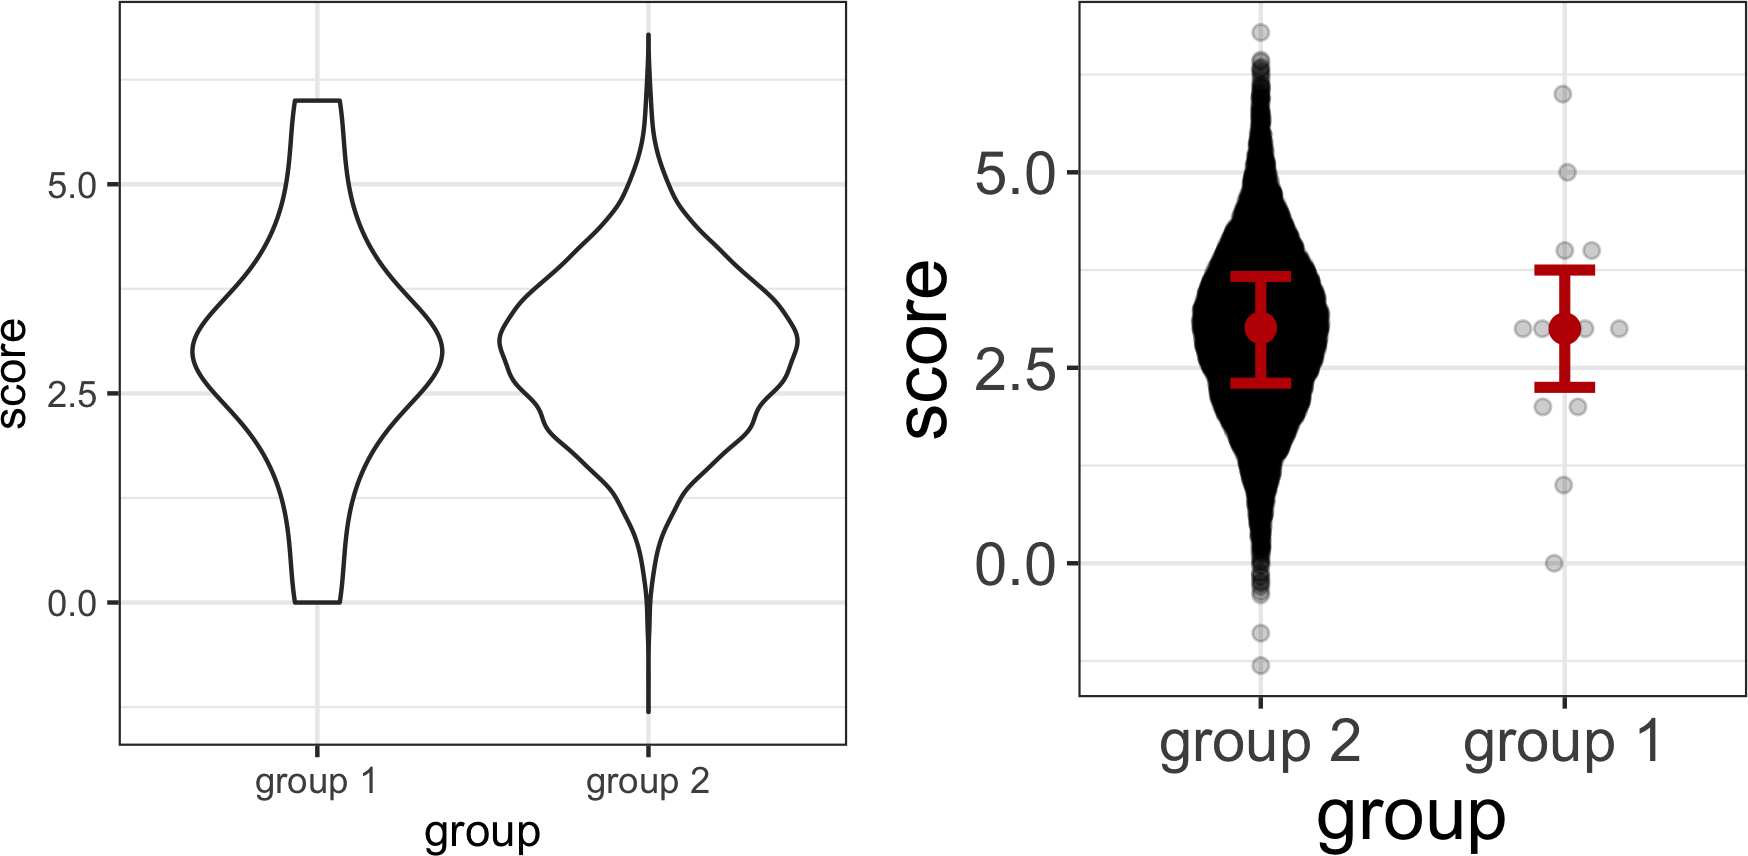
\includegraphics[width=0.9\linewidth]{flexplot_manual_files/figure-latex/raw-1} 

}

\caption{Violin plots with 15,000 versus 15 datapoints. The outlines look the same in the left image, but the right image overlays the raw data, which makes the differing sample sizes much more apparent.}\label{fig:raw}
\end{figure}

In \texttt{flexplot()}, one can control the amount of jittering. The
amount of jittering can be specified in multiple ways: as a boolean
(\texttt{TRUE} means it will jitter, \texttt{FALSE} it won't), as a
number (e.g., \texttt{0.2}), or as a vector (e.g., \texttt{c(.2,\ .4)},
which will indicate .2 jittering for X and .4 for Y). Just as it is in
\texttt{geom\_jitter()}, this number refers to the amount of jittering
on either side. However, the value refers to the \emph{maximum} amount
the computer will jitter the data. So, 0.2 (the default) will jitter
10\% of the way to the right only at the highest density and 10\% to the
left at the highest density.

Users can also specify what the ``whiskers'' mean for the summary
statistics. They default to the interquartile range (with the median as
the center dot), but the user can also specify \texttt{sterr}, or
\texttt{stdev,} to indicate the standard error or standard deviation:

\begin{Shaded}
\begin{Highlighting}[]
\KeywordTok{data}\NormalTok{(}\StringTok{"exercise_data"}\NormalTok{)}
\NormalTok{a =}\StringTok{ }\KeywordTok{flexplot}\NormalTok{(weight.loss}\OperatorTok{~}\NormalTok{therapy.type, }\DataTypeTok{data=}\NormalTok{exercise_data, }
             \DataTypeTok{jitter=}\NormalTok{F, }\DataTypeTok{spread=}\StringTok{"quartile"}\NormalTok{)}
\NormalTok{b =}\StringTok{ }\KeywordTok{flexplot}\NormalTok{(weight.loss}\OperatorTok{~}\NormalTok{therapy.type, }\DataTypeTok{data=}\NormalTok{exercise_data, }
             \DataTypeTok{jitter=}\KeywordTok{c}\NormalTok{(.}\DecValTok{4}\NormalTok{,.}\DecValTok{5}\NormalTok{), }\DataTypeTok{spread=}\StringTok{"sterr"}\NormalTok{)}
\NormalTok{c =}\StringTok{ }\KeywordTok{flexplot}\NormalTok{(weight.loss}\OperatorTok{~}\NormalTok{therapy.type, }\DataTypeTok{data=}\NormalTok{exercise_data, }
             \DataTypeTok{jitter=}\NormalTok{.}\DecValTok{2}\NormalTok{, }\DataTypeTok{spread=}\StringTok{"stdev"}\NormalTok{)}
\NormalTok{cowplot}\OperatorTok{::}\KeywordTok{plot_grid}\NormalTok{(a,b,c, }\DataTypeTok{nrow=}\DecValTok{1}\NormalTok{)}
\end{Highlighting}
\end{Shaded}

\begin{figure}

{\centering \includegraphics[width=0.9\linewidth]{flexplot_manual_files/figure-latex/unnamed-chunk-2-1} 

}

\caption{Dot plots with IQR and no jittering (left), JD plot with mean + standard errors + jittering on $X$ and $Y$ (middle), and JD plot with mean + standard deviation with jittering on only $X$ (right), as well as different forms of jittering.}\label{fig:unnamed-chunk-2}
\end{figure}

\section*{Numeric Predictor, Numeric Outcome
(Scatterplots)}\label{numeric-predictor-numeric-outcome-scatterplots}
\addcontentsline{toc}{section}{Numeric Predictor, Numeric Outcome
(Scatterplots)}

The indisputed king of numeric on numeric visualization is the
scatterplot. Once again, \texttt{flexplot()} is smart enough to know to
plot a scatterplot when it is passed a numeric predictor. The fit of the
graph defaults to a loess line, so as to highlight deviations from
linearity. However, the user can specify other sorts of fits, such as
\texttt{"lm"} (for regression), \texttt{"polynomial"}, \texttt{"cubic"},
and \texttt{"rlm"} (robust linear models). The user can also choose to
remove the confidence interval by specifying \texttt{se=F}, as well as
jitter one or both variables, as shown below.

\begin{Shaded}
\begin{Highlighting}[]
\KeywordTok{data}\NormalTok{(}\StringTok{"exercise_data"}\NormalTok{)}
\NormalTok{a =}\StringTok{ }\KeywordTok{flexplot}\NormalTok{(weight.loss}\OperatorTok{~}\NormalTok{satisfaction, }\DataTypeTok{data=}\NormalTok{exercise_data)}
\NormalTok{b =}\StringTok{ }\KeywordTok{flexplot}\NormalTok{(weight.loss}\OperatorTok{~}\NormalTok{satisfaction, }\DataTypeTok{data=}\NormalTok{exercise_data, }
             \DataTypeTok{method=}\StringTok{"lm"}\NormalTok{, }\DataTypeTok{se=}\NormalTok{F)}
\NormalTok{c =}\StringTok{ }\KeywordTok{flexplot}\NormalTok{(weight.loss}\OperatorTok{~}\NormalTok{satisfaction, }\DataTypeTok{data=}\NormalTok{exercise_data, }
             \DataTypeTok{method=}\StringTok{"polynomial"}\NormalTok{, }\DataTypeTok{jitter=}\NormalTok{.}\DecValTok{4}\NormalTok{)}
\NormalTok{cowplot}\OperatorTok{::}\KeywordTok{plot_grid}\NormalTok{(a,b,c, }\DataTypeTok{nrow=}\DecValTok{1}\NormalTok{)}
\end{Highlighting}
\end{Shaded}

\begin{figure}

{\centering 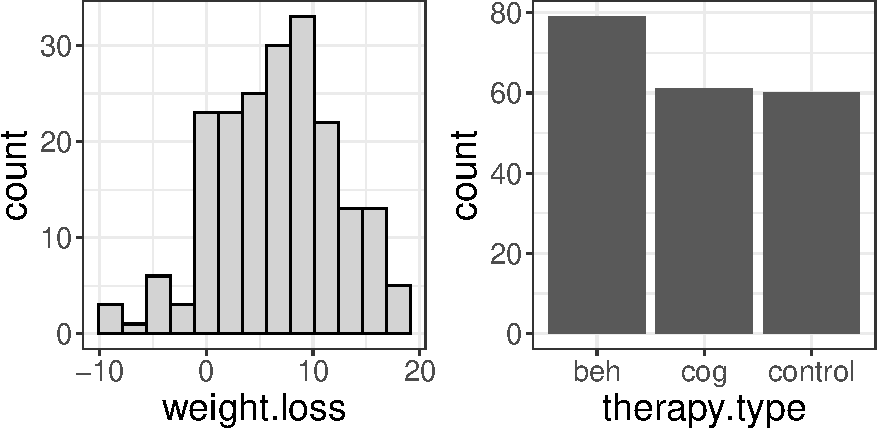
\includegraphics[width=0.9\linewidth]{flexplot_manual_files/figure-latex/unnamed-chunk-3-1} 

}

\caption{Scatterplot with different options of fit: loess (default), lm (regression), polynomial}\label{fig:unnamed-chunk-3}
\end{figure}

\section*{Numeric Predictor, Categorical Outcome (Logistic
Curves)}\label{numeric-predictor-categorical-outcome-logistic-curves}
\addcontentsline{toc}{section}{Numeric Predictor, Categorical Outcome
(Logistic Curves)}

\texttt{flexplot()} also has some ability to model categorical outcomes.
One common situation might be when one is attempting to model a binary
outcome, as they would in a logistic regression. Any binary variable can
be visualized as a logistic regression in Flexplot, except when the axis
variable is also numeric (i.e., the variable occupying the first slot in
the \texttt{flexplot()} equation. To do so, the user only needs to
specify \texttt{logistic} as the method.

\begin{Shaded}
\begin{Highlighting}[]
\KeywordTok{data}\NormalTok{(}\StringTok{"tablesaw.injury"}\NormalTok{)}
\KeywordTok{require}\NormalTok{(dplyr)}
\KeywordTok{flexplot}\NormalTok{(injury}\OperatorTok{~}\NormalTok{attention, }\DataTypeTok{data=}\NormalTok{tablesaw.injury, }
             \DataTypeTok{method=}\StringTok{"logistic"}\NormalTok{, }\DataTypeTok{jitter=}\KeywordTok{c}\NormalTok{(}\DecValTok{0}\NormalTok{, .}\DecValTok{05}\NormalTok{))}
\end{Highlighting}
\end{Shaded}

\section*{Categorical Outcome, Categorical Predictor (Association
Plots)}\label{categorical-outcome-categorical-predictor-association-plots}
\addcontentsline{toc}{section}{Categorical Outcome, Categorical
Predictor (Association Plots)}

Sometimes the analyst may wish to visualize the relationship between two
categorical variables. Once again, \texttt{flexplot()} is smart enough
to determine that information from the formula, provided the user
supplied two factors. In this situation, \texttt{flexplot()} will
generate an ``association'' plot, which plots the deviation each cell
from its expected frequencies (divided by the expected values of that
cell). will In the example below, I had to convert \texttt{injury} to a
factor to get a barplot. The graphic shows that females are less likely
to be injured than males, relatively speaking.

\begin{Shaded}
\begin{Highlighting}[]
\NormalTok{tablesaw.injury}\OperatorTok{$}\NormalTok{injury =}\StringTok{ }\KeywordTok{factor}\NormalTok{(tablesaw.injury}\OperatorTok{$}\NormalTok{injury, }
                                \DataTypeTok{levels=}\KeywordTok{c}\NormalTok{(}\DecValTok{0}\NormalTok{,}\DecValTok{1}\NormalTok{), }\DataTypeTok{labels=}\KeywordTok{c}\NormalTok{(}\StringTok{"all good"}\NormalTok{, }\StringTok{"ouch"}\NormalTok{))}
\KeywordTok{flexplot}\NormalTok{(injury}\OperatorTok{~}\NormalTok{gender, }\DataTypeTok{data=}\NormalTok{tablesaw.injury)}
\end{Highlighting}
\end{Shaded}

\section*{Repeated Measures Data (Related
T-Test)}\label{repeated-measures-data-related-t-test}
\addcontentsline{toc}{section}{Repeated Measures Data (Related T-Test)}

As I mentioned previously, one of the guiding tenets of Flexplot is that
every statistical analysis ought to be accompanied by a graphic that
closely matches the analysis. With a related t-test, the existing
graphics will not accurately represent this model because a related t
actually models the \emph{difference} between scores (e.g., from Time 1
to Time 2). As such, \texttt{flexplot()} allows an additional option
(\texttt{related\ =\ TRUE}) that tells \texttt{flexplot()} to plot the
differences, rather than the groups. To do so, \texttt{flexplot()}
requires ``tidy'' data, or data where Time is indicated in one column
and the score in the other. Once in this format, it simply plots the
differences. For example:

\begin{Shaded}
\begin{Highlighting}[]
\KeywordTok{data}\NormalTok{(}\StringTok{"plant_growth"}\NormalTok{)}
\KeywordTok{flexplot}\NormalTok{(Diameter}\OperatorTok{~}\NormalTok{Soil.Type, }\DataTypeTok{data=}\NormalTok{plant_growth, }\DataTypeTok{related=}\NormalTok{T)}
\end{Highlighting}
\end{Shaded}

\noindent (Note, this dataset didn't actually contain repeated measures
data. This is merely for illustrative purposes).

Unfortunately, plotting difference scores only works with two
timepoints. When there are more than two timepoints, I recommend
visualizing these relationships with the \texttt{visualize()} function
for a mixed model. (I'll address \texttt{visualize()} shortly). In the
plant growth graphic, the differences seem centered around zero,
indicating that the type of soil used (store-bought potting soil versus
a ``secret'' custom mix I found online) didn't make a difference.

\section*{Avoiding Overlap}\label{avoiding-overlap}
\addcontentsline{toc}{section}{Avoiding Overlap}

If it wasn't yet apparent, let me be less subtle: I think all graphics
should include raw data. Showing raw data allows readers to determine
whether the chosen model is appropriate, and it communicates the degree
of uncertainty about the model. However, when there are a very large
number of datapoints, it becomes quite difficult to see any patterns;
areas of high density look just as crowded as areas of lower density,
relatively speaking (although having JD plots makes it clear which areas
are most dense; see the example in top-left image in Figure
@ref(fig:sample\}). To address such overlap, \texttt{flexplot()} offers
three options. The first is to suppress raw data (\texttt{raw.data=F},
right image on top). I don't recommend that, but it can be done. A
second option is to reduce the transparency (e.g.,
\texttt{alpha\ =\ 0.2}, bottom-left image). Perhaps the best option is
to \emph{sample} (bottom-right). However, it is important that the
visual display of fit (e.g., median + IQR, loess line, regression line)
not be generated from the sampled data. Rather, the fit should
correspond to the entire dataset. \texttt{flexplot()} performs this
operation in the background. In Figure @ref(fig:sample\}, notice how the
medians/interquartile ranges do not change, despite having different
numbers of datapoints.

\begin{Shaded}
\begin{Highlighting}[]
\KeywordTok{data}\NormalTok{(}\StringTok{"nsduh"}\NormalTok{)}

\NormalTok{a =}\StringTok{ }\KeywordTok{flexplot}\NormalTok{(distress}\OperatorTok{~}\NormalTok{major.dep, }\DataTypeTok{data=}\NormalTok{nsduh)}
\NormalTok{b =}\StringTok{ }\KeywordTok{flexplot}\NormalTok{(distress}\OperatorTok{~}\NormalTok{major.dep, }\DataTypeTok{data=}\NormalTok{nsduh, }\DataTypeTok{raw.data=}\NormalTok{F)}
\NormalTok{c =}\StringTok{ }\KeywordTok{flexplot}\NormalTok{(distress}\OperatorTok{~}\NormalTok{major.dep, }\DataTypeTok{data=}\NormalTok{nsduh, }\DataTypeTok{alpha=}\NormalTok{.}\DecValTok{005}\NormalTok{)}
\NormalTok{d =}\StringTok{ }\KeywordTok{flexplot}\NormalTok{(distress}\OperatorTok{~}\NormalTok{major.dep, }\DataTypeTok{data=}\NormalTok{nsduh, }\DataTypeTok{sample=}\DecValTok{200}\NormalTok{)}

\NormalTok{cowplot}\OperatorTok{::}\KeywordTok{plot_grid}\NormalTok{(a,b,c,d, }\DataTypeTok{nrow=}\DecValTok{2}\NormalTok{)}
\end{Highlighting}
\end{Shaded}

\begin{figure}
\centering
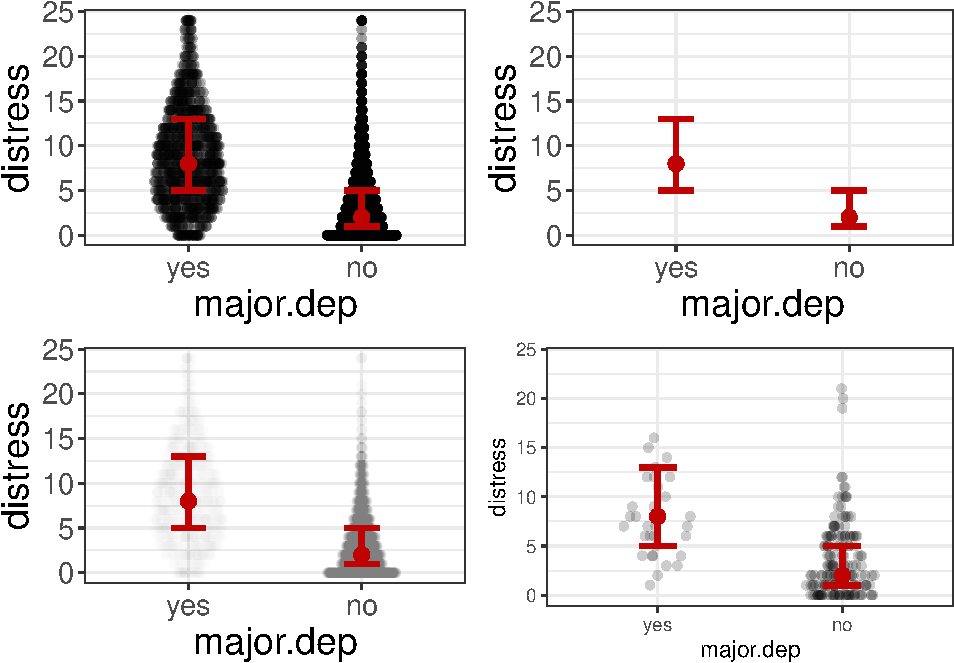
\includegraphics{flexplot_manual_files/figure-latex/sample-1.pdf}
\caption{\label{fig:sample}Four graphics showing different ways to handle
overlapping datapoints. The far left image does nothing. The second from
the left does not include raw data. The third reduces the opacity. The
fourth samples.}
\end{figure}

\chapter*{Multivariate Graphics}\label{multivariate-graphics}
\addcontentsline{toc}{chapter}{Multivariate Graphics}

Visualizing multivariate relationships can become quite tricky. It is
very easy to experience cognitive overload, especially when one is
attempting to visualize raw data (which is, again, a key characteristic
of Flexplot). Some might be inclined to do three-dimensional plots.
However, I find these difficult to interpret and they require the user
to rotate the view. Even then, they can only show two two predictors at
a time. I find it much easier to use other strategies.
\texttt{flexplot()} utilizes four different strategies to visualize
multivariate relationships: (1) plotting a dimension as different
colors/lines/shapes, (2) plotting a dimension in row or column panels,
(3) visualize conditional relationships with added variable plots, and
(4) overlaying ghost lines.

\section*{Added Variable Plots (AVPs)}\label{added-variable-plots-avps}
\addcontentsline{toc}{section}{Added Variable Plots (AVPs)}

AVPs are underused, yet extremely useful. Essentially, an AVP shows the
relationship between a predictor of interest and the \emph{residuals} of
an existing model. For example, if one wanted to understand the
relationship between \texttt{therapy.type} and \texttt{weight.loss}
after controlling for motivation, that person could build a model
predicting weight loss from motivation, residualize that relationship,
then show a JD plot of the residuals for each type of therapy. This is
what AVP's do (see Figure @ref(fig:avp\}). Flexplot's version of AVPs
have a slightly different flavor. In my experience, AVPs can be
confusing because the scale of the outcome variable has changed. To
counter this confusing, Flexplot adds the mean back into the residuals
so the \(Y\)-axis retains the original scale. The notation for
\texttt{added.plot()} is similar to \texttt{flexplot()}, though the
vertical pipes aren't necessary. What \texttt{flexplot()} will do is
take the \emph{last} variable entered (\texttt{therapy.type} in the
following example) and plot that on the \(X\) axis, while plotting the
residuals of the model predicting the outcome (\texttt{weight.loss} in
this case) from the other variable(s) in the model (\texttt{motivation},
in this case). Other arguments can be passed to \texttt{added.plots()}
as well (such as alpha, sample, method, etc.)

\begin{Shaded}
\begin{Highlighting}[]
\KeywordTok{data}\NormalTok{(}\StringTok{"exercise_data"}\NormalTok{)}
\KeywordTok{added.plot}\NormalTok{(weight.loss}\OperatorTok{~}\NormalTok{motivation }\OperatorTok{+}\StringTok{ }\NormalTok{therapy.type, }\DataTypeTok{data=}\NormalTok{exercise_data)}
\end{Highlighting}
\end{Shaded}

The advantage of AVPs is that they match almost exactly what a multiple
regression is doing. The parameters (as well as tests of significance)
reflect the added contribution of that particular variable, after
controlling for all other variables in the model. (Technically, AVPs are
not an exact match because regression models perform these
simultaneously, while AVPs perform these calculations in sequence).
However, one major limitation of AVPs is that they show the conditional
relationship of the variable of interest after controlling for the
\emph{linear main effects} of the other variable(s) in the model. If any
nonlinear and/or interactions are present in the model, AVPs will give a
biased representation of the residualized effect. For example, if there
was a strong interaction between \texttt{therapy.type} and
\texttt{motivation} and/or the relationship between \texttt{motivation}
and \texttt{weight.loss} is curvilinear, AVPs give an inaccurate
representation of the data. As an aside, the same applies for any
multiple regression model. No parameter should be interpreted if
nonlinear and/or interaction terms exist between predictor variables and
the outcome.

On the other hand, AVPs are extremely easy to interpret. As such, when
visualizing multivariate relationships, I first look for evidence there
are no interactions and/or nonlinear patterns in the data so I can
visualize the AVPs.

\section*{Colors/Lines/Shapes}\label{colorslinesshapes}
\addcontentsline{toc}{section}{Colors/Lines/Shapes}

As shown in Figure xxx, the second slot in the \texttt{flexplot()}
formula (\texttt{X2} in Figure xx) controls which variable will be
displayed using a different colors/symbols/lines. Figure
\ref{fig:symbols} shows two examples of this: one where a numeric
predictor is on the \(X\) axis, and one where a categorical predictor is
on the X-axis. When categorical variables are shown on the X-axis,
\texttt{flexplot()} draws lines connecting the medians (or means).

\begin{Shaded}
\begin{Highlighting}[]
\NormalTok{a =}\StringTok{ }\KeywordTok{flexplot}\NormalTok{(weight.loss}\OperatorTok{~}\NormalTok{motivation }\OperatorTok{+}\StringTok{ }\NormalTok{gender, }\DataTypeTok{data=}\NormalTok{exercise_data, }\DataTypeTok{se=}\NormalTok{F)}
\NormalTok{b =}\StringTok{ }\KeywordTok{flexplot}\NormalTok{(weight.loss}\OperatorTok{~}\NormalTok{therapy.type }\OperatorTok{+}\StringTok{ }\NormalTok{gender, }\DataTypeTok{data=}\NormalTok{exercise_data, }\DataTypeTok{se=}\NormalTok{F)}
\NormalTok{cowplot}\OperatorTok{::}\KeywordTok{plot_grid}\NormalTok{(a,b)}
\end{Highlighting}
\end{Shaded}

\begin{figure}

{\centering 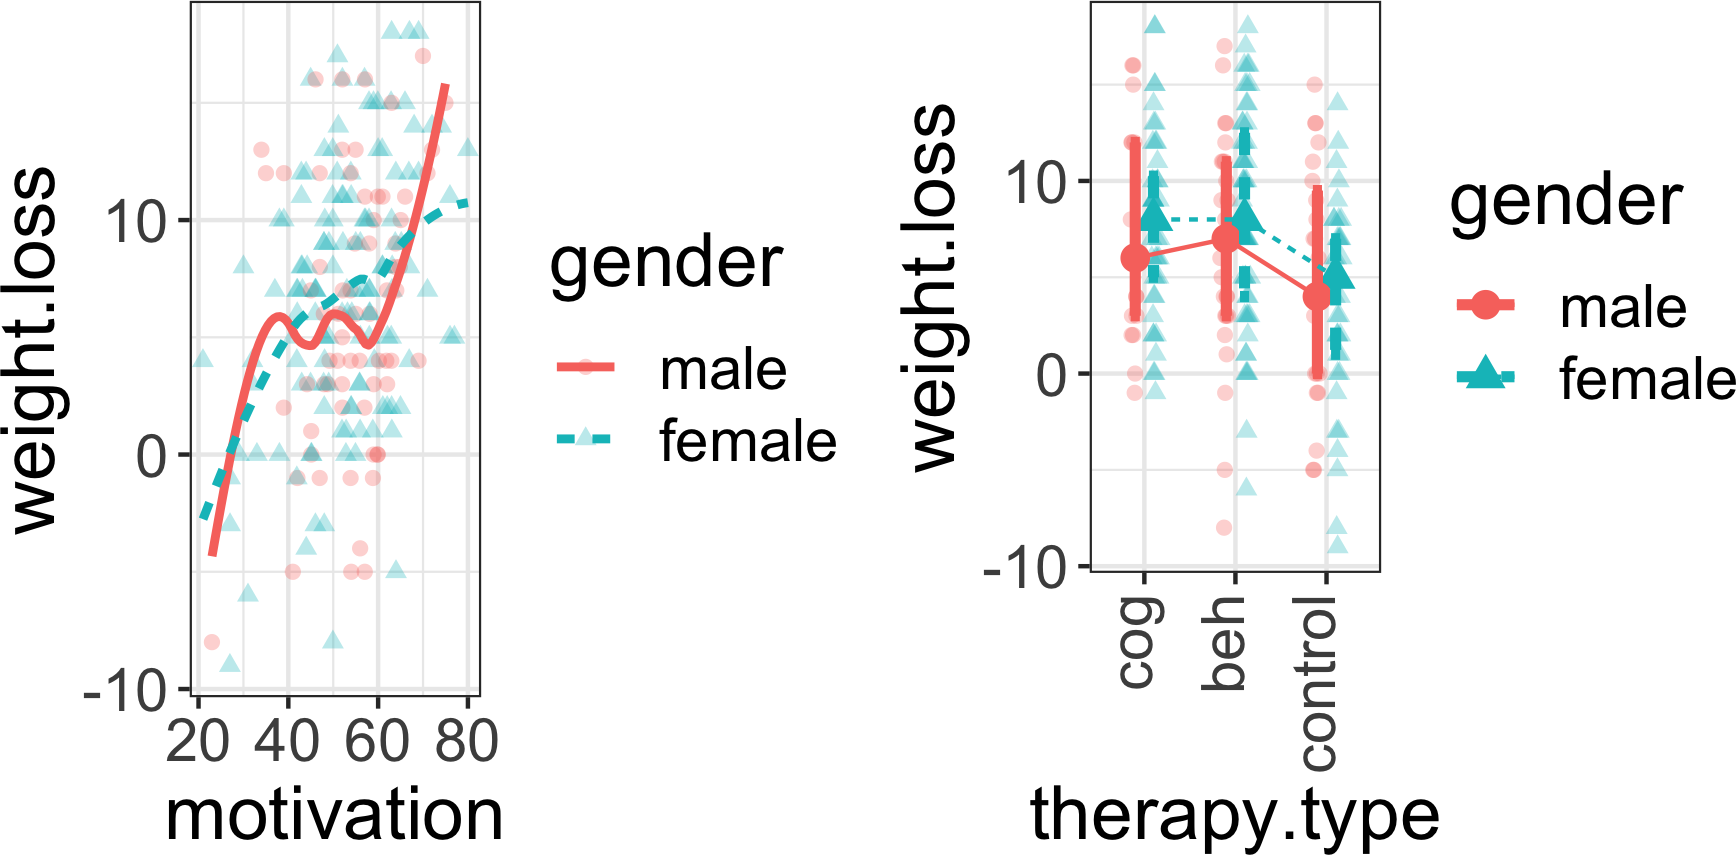
\includegraphics[width=0.9\linewidth]{flexplot_manual_files/figure-latex/symbols-1} 

}

\caption{A multivariate plot with therapy.type showing as separate lines/colors/symbols, with confidence interval bands removed.}\label{fig:symbols}
\end{figure}

One limitation of colors/shapes/symbols is the increase cognitive load.
When plotting different symbols/colors/lines on the same graph, there is
often a great deal of overlap, which makes it more difficult to pick out
patterns. In my experience, having a variable with more than two levels
in the second slot of a \texttt{flexplot()} equation becomes challenging
to interpret, particularly when there are more than a handful of
datapoints.

\section*{Paneling}\label{paneling}
\addcontentsline{toc}{section}{Paneling}

An alternative (or additional) strategy for plotting multivariate data
is paneling. As shown in Figure xx, the third and fourth slots control
paneling in columns and rows, respectively. The panels follow many
conventions created by William Cleveland (1994), such as having the
first variable control the columns, and having values increase from left
to right and bottom to top (just as they do on the \(X\) and \(Y\) axis,
respectively).

Figure \ref{fig:panels} shows the same relationships in Figure
\ref{fig:symbols}, but with the second variable in panels instead. The
far right image also displays panels for three variables simultaneously.
Paneled variables are easy to conceptualize with categorical variables,
but what about numeric variables? These can still be visualized, but the
values must be binned. Also notice that I have taken advantage of the
fact that \texttt{flexplot()} returns a \texttt{ggplot2} object that can
be edited. (In this case, I'm modifying the behavior of the labels to
prevent cutting them off).\footnote{I also do not show the code where I
  actually plot the graphics. This required some advanced manipulation
  of the layout and I didn't want to detract from what
  \texttt{flexplot()} is doing.}

\begin{Shaded}
\begin{Highlighting}[]
\NormalTok{a =}\StringTok{ }\KeywordTok{flexplot}\NormalTok{(weight.loss}\OperatorTok{~}\NormalTok{motivation }\OperatorTok{|}\StringTok{ }\NormalTok{gender, }
             \DataTypeTok{data=}\NormalTok{exercise_data)}
\NormalTok{b =}\StringTok{ }\KeywordTok{flexplot}\NormalTok{(weight.loss}\OperatorTok{~}\NormalTok{therapy.type }\OperatorTok{|}\StringTok{ }\NormalTok{gender, }
             \DataTypeTok{data=}\NormalTok{exercise_data)}
\NormalTok{c =}\StringTok{ }\KeywordTok{flexplot}\NormalTok{(weight.loss}\OperatorTok{~}\NormalTok{motivation }\OperatorTok{|}\StringTok{  }\NormalTok{gender }\OperatorTok{+}\StringTok{ }\NormalTok{therapy.type, }
             \DataTypeTok{data=}\NormalTok{exercise_data) }\OperatorTok{+}
\StringTok{      }\NormalTok{ggplot2}\OperatorTok{::}\KeywordTok{facet_grid}\NormalTok{(therapy.type}\OperatorTok{~}\NormalTok{gender, }
                          \DataTypeTok{labeller =}\NormalTok{ ggplot2}\OperatorTok{::}\KeywordTok{labeller}\NormalTok{(}\DataTypeTok{therapy.type=}\NormalTok{label_value))}
\end{Highlighting}
\end{Shaded}

\begin{figure}

{\centering 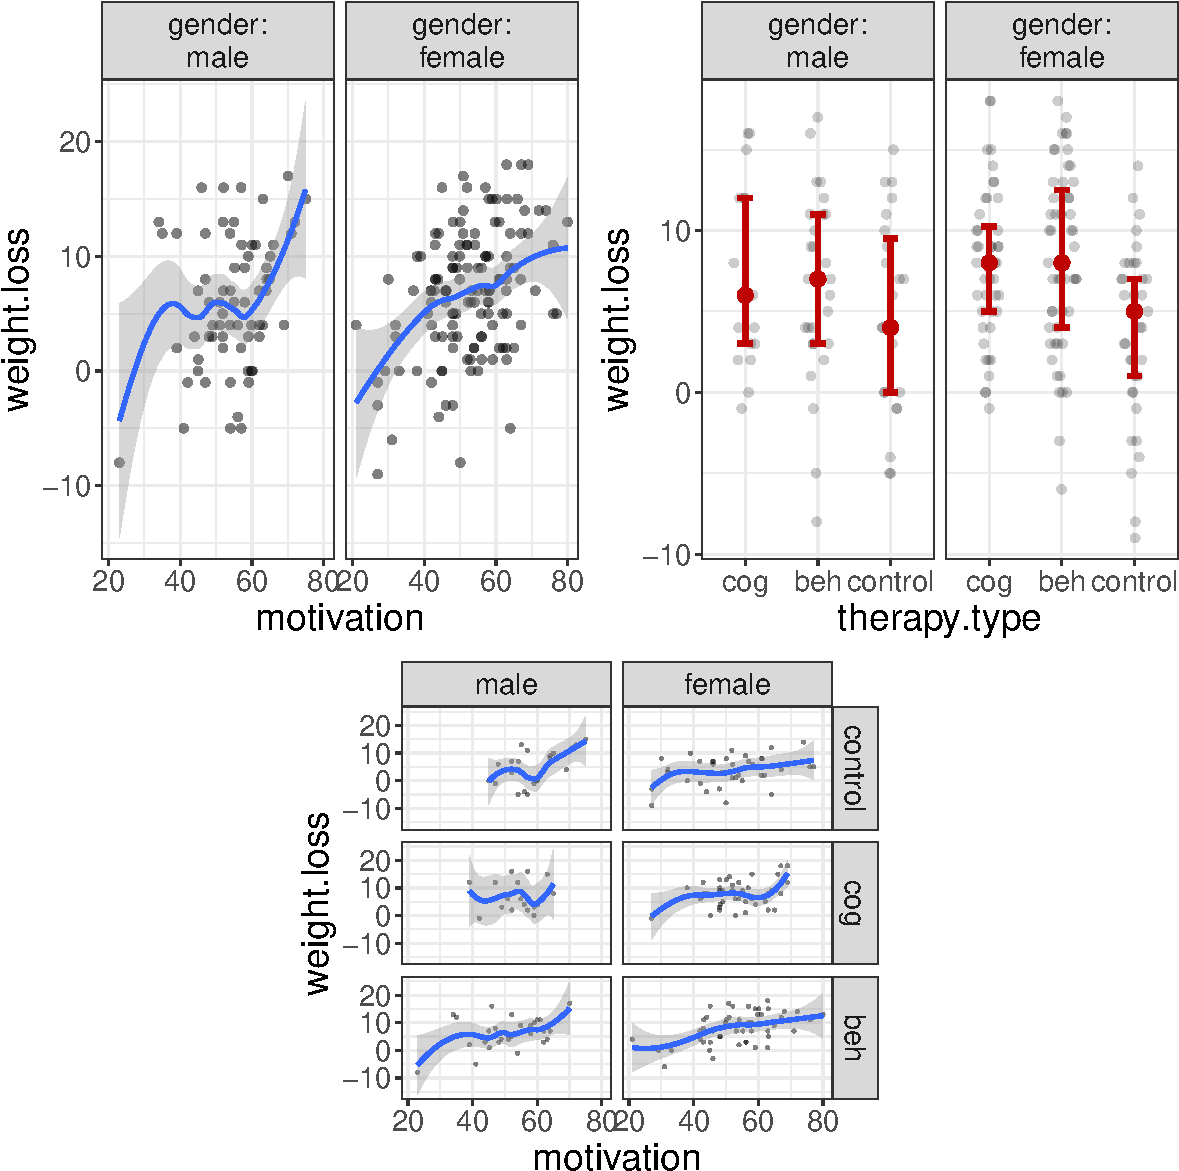
\includegraphics[width=0.9\linewidth]{flexplot_manual_files/figure-latex/panels-1} 

}

\caption{A multivariate plot where `therapy.type` and `gender` are now shown in panels.}\label{fig:panels}
\end{figure}

\section*{Binning}\label{binning}
\addcontentsline{toc}{section}{Binning}

Within \texttt{flexplot()}, any numeric predictor, with the exception of
the variable in the first slot, will be binned into discrete categories.
These bins will then be represented in panels (if the variable is in the
third or fourth slot) or as colors/symbols/lines (if the variable is in
the second slot). The user has the option of specifying the number of
bins (e.g., 2 or 3), or the user can specify breakpoints at which to
bin. When the user specifies bins, \texttt{flexplot()} will attempt to
have an equal number of datapoints in each bin. However,
\texttt{flexplot()} may be unable to bin into the specified number of
bins. For example, if a user specifies four bins, it's possible the
scores at the 50th and 75th percentile are the same. In these cases,
\texttt{flexplot()} will choose a smaller bin number, though it will
report such to the user. \texttt{flexplot()} defaults to three bins.

When specifying breakpoints, the panels may have different sample sizes
in each bin. A user may wish to do this if these breakpoints are
meaningful (e.g., when particular scores are clinically meaningful, such
as Beck Depression Inventory scores above 29 are considered severly
depressed).

Whether using breakpoints, or bins, the user can also specify labels for
the bins. Figure \ref{fig:panels2}shows three plots of the same
variables: the first specifies two breakpoints, the second specifies two
bins with labels, and the third just specifies the bins.

\begin{Shaded}
\begin{Highlighting}[]
\NormalTok{a =}\StringTok{ }\KeywordTok{flexplot}\NormalTok{(weight.loss}\OperatorTok{~}\NormalTok{motivation }\OperatorTok{|}\StringTok{ }\NormalTok{satisfaction, }
             \DataTypeTok{data=}\NormalTok{exercise_data, }
             \DataTypeTok{breaks=}\KeywordTok{list}\NormalTok{(}\DataTypeTok{satisfaction=}\KeywordTok{c}\NormalTok{(}\DecValTok{3}\NormalTok{,}\DecValTok{7}\NormalTok{))) }
\NormalTok{b =}\StringTok{ }\KeywordTok{flexplot}\NormalTok{(weight.loss}\OperatorTok{~}\NormalTok{motivation }\OperatorTok{+}\StringTok{ }\NormalTok{satisfaction, }
             \DataTypeTok{data=}\NormalTok{exercise_data, }
             \DataTypeTok{breaks=}\KeywordTok{list}\NormalTok{(}\DataTypeTok{satisfaction=}\KeywordTok{c}\NormalTok{(}\DecValTok{3}\NormalTok{,}\DecValTok{7}\NormalTok{)), }
             \DataTypeTok{labels=}\KeywordTok{list}\NormalTok{(}\DataTypeTok{satisfaction=}\KeywordTok{c}\NormalTok{(}\StringTok{"low"}\NormalTok{, }\StringTok{"medium"}\NormalTok{, }\StringTok{"high"}\NormalTok{)))}

\NormalTok{c =}\StringTok{ }\KeywordTok{flexplot}\NormalTok{(weight.loss}\OperatorTok{~}\NormalTok{motivation }\OperatorTok{+}\StringTok{ }\NormalTok{satisfaction, }
             \DataTypeTok{data=}\NormalTok{exercise_data, }
             \DataTypeTok{bins=}\DecValTok{2}\NormalTok{) }
\end{Highlighting}
\end{Shaded}

\begin{Shaded}
\begin{Highlighting}[]
\NormalTok{  top.row =}\StringTok{ }\NormalTok{cowplot}\OperatorTok{::}\KeywordTok{plot_grid}\NormalTok{(a,b, }\DataTypeTok{ncol=}\DecValTok{2}\NormalTok{, }\DataTypeTok{rel_widths=}\KeywordTok{c}\NormalTok{(}\DecValTok{1}\NormalTok{,}\FloatTok{1.5}\NormalTok{))}
\NormalTok{  bottom.row =}\StringTok{ }\NormalTok{cowplot}\OperatorTok{::}\KeywordTok{plot_grid}\NormalTok{(}\OtherTok{NULL}\NormalTok{, c, }\OtherTok{NULL}\NormalTok{, }\DataTypeTok{ncol=}\DecValTok{3}\NormalTok{, }\DataTypeTok{rel_widths=}\KeywordTok{c}\NormalTok{(.}\DecValTok{2}\NormalTok{, .}\DecValTok{6}\NormalTok{,.}\DecValTok{2}\NormalTok{))}
\NormalTok{  cowplot}\OperatorTok{::}\KeywordTok{plot_grid}\NormalTok{(top.row, bottom.row, }\DataTypeTok{nrow=}\DecValTok{2}\NormalTok{,}\DataTypeTok{rel_heights =} \KeywordTok{c}\NormalTok{(.}\DecValTok{55}\NormalTok{, .}\DecValTok{45}\NormalTok{))}
\end{Highlighting}
\end{Shaded}

\begin{figure}

{\centering 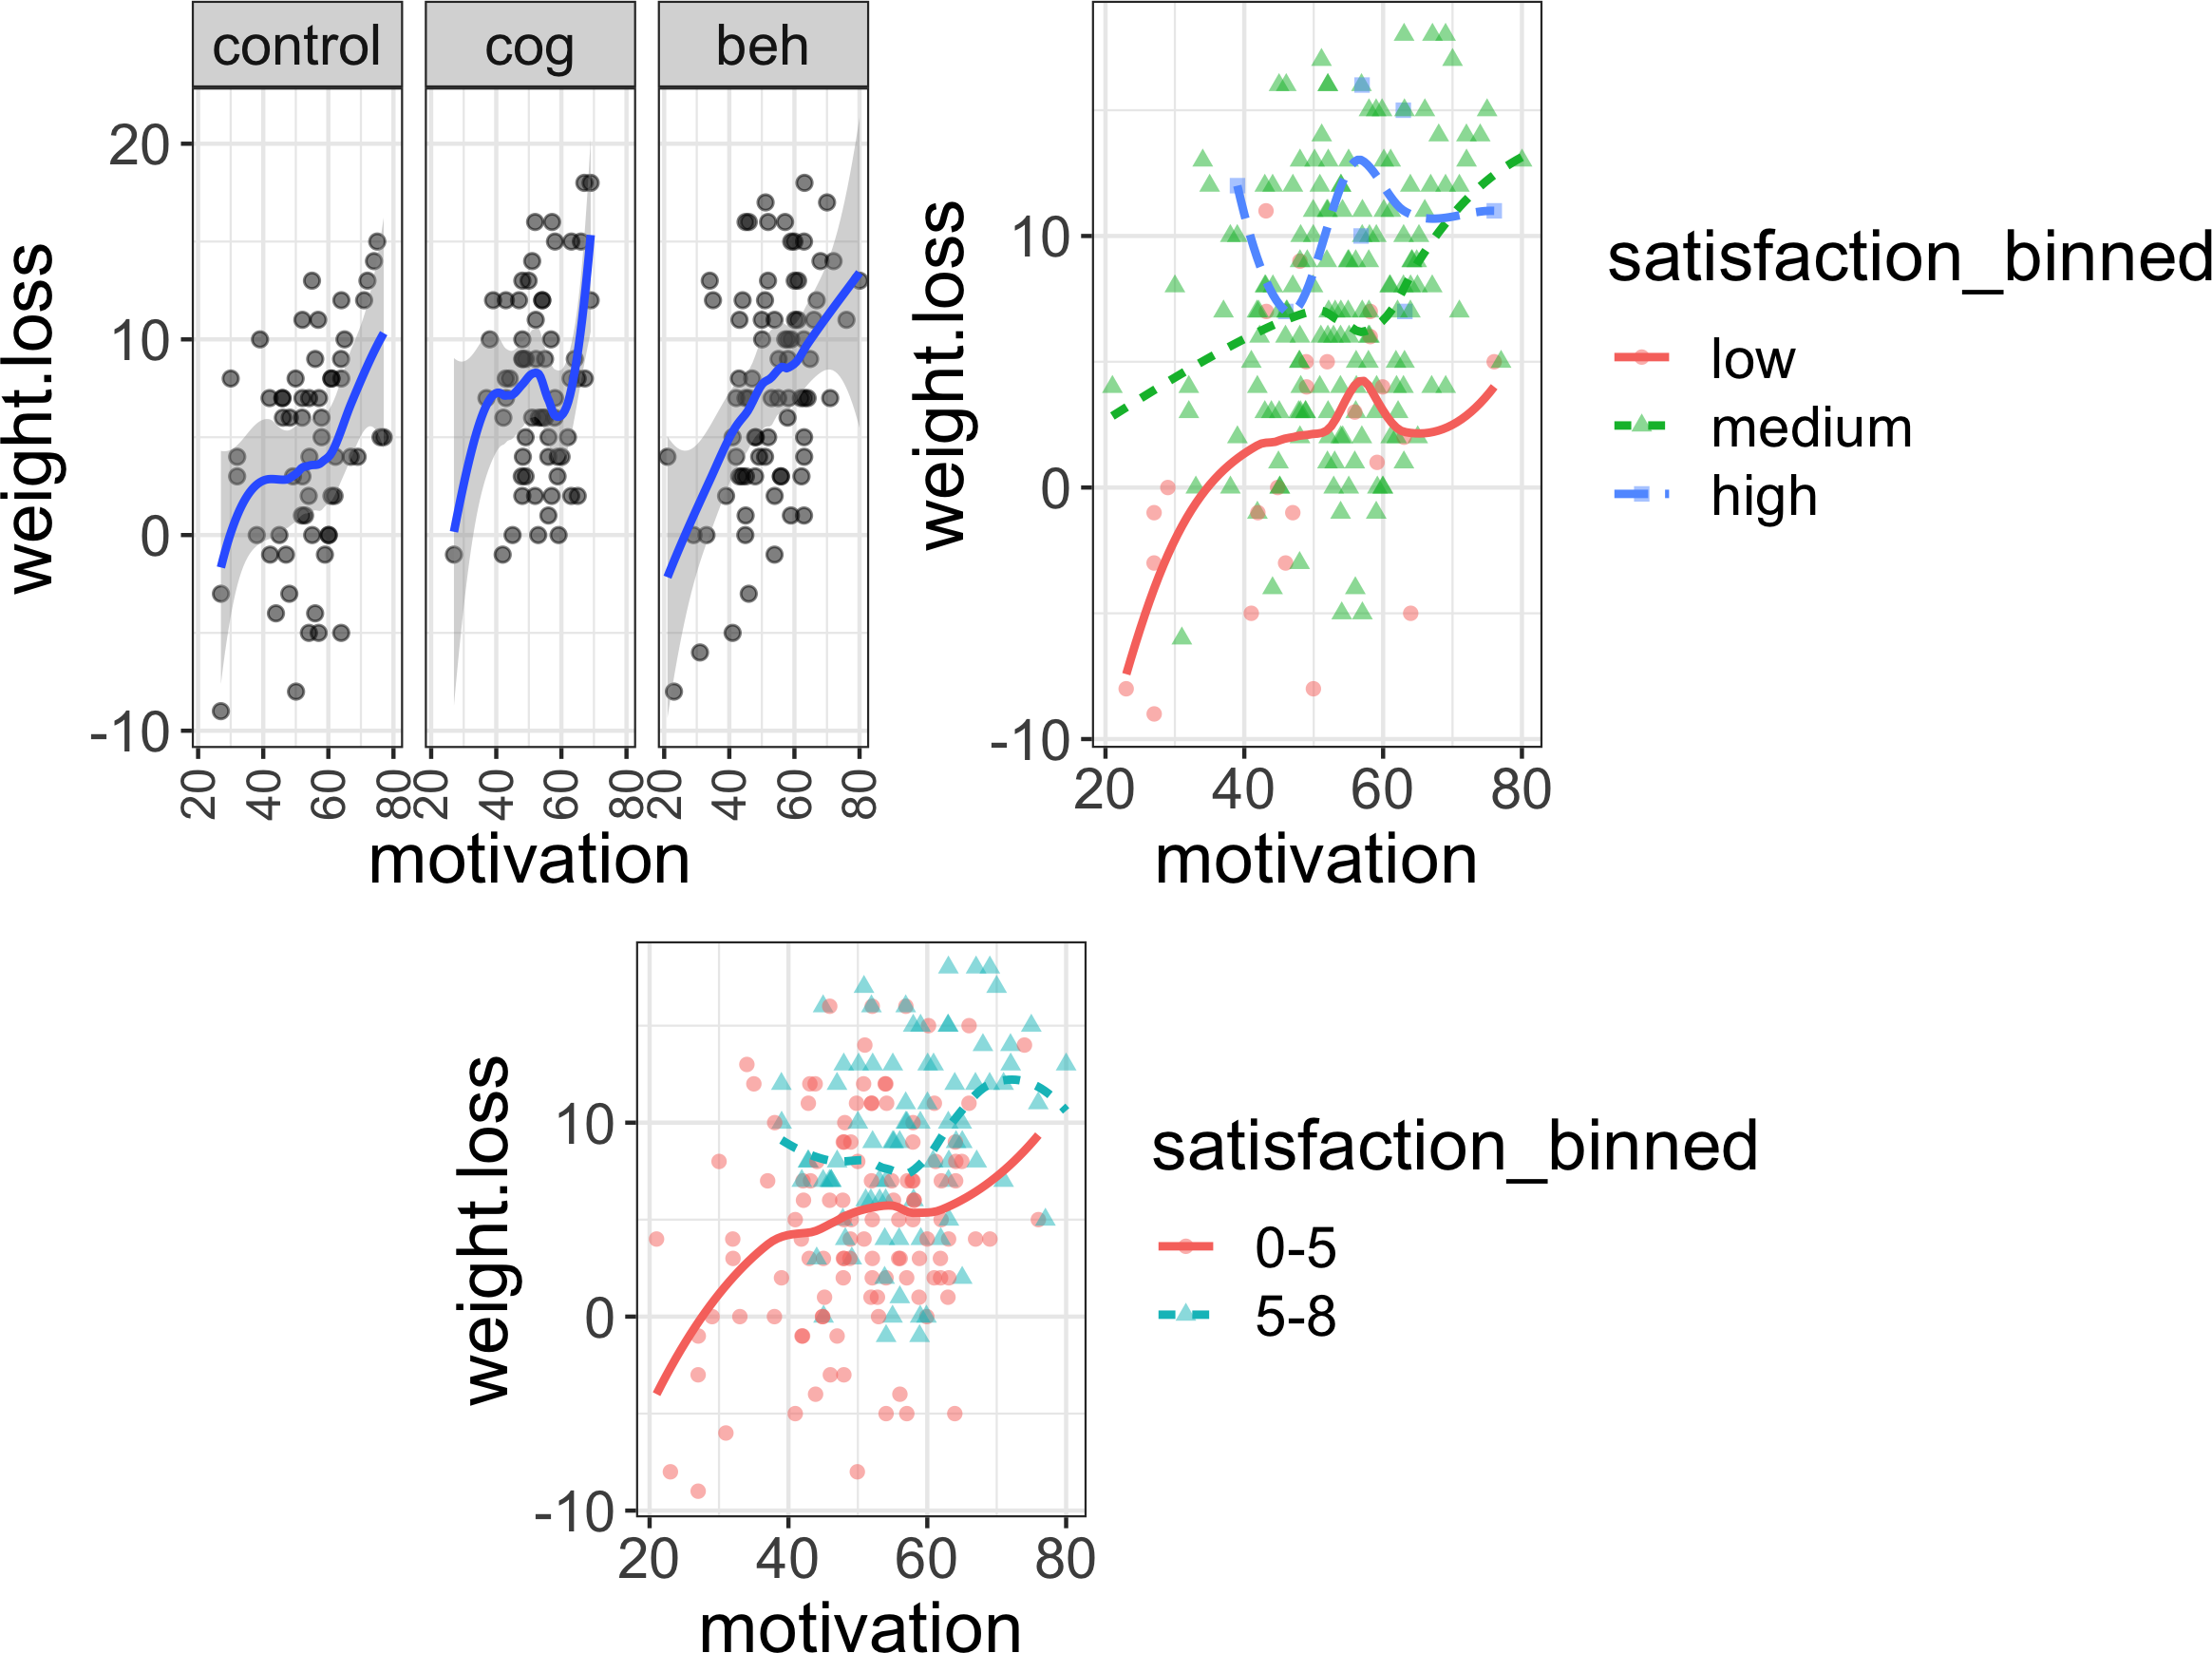
\includegraphics[width=0.9\linewidth]{flexplot_manual_files/figure-latex/panels2-1} 

}

\caption{Demonstration of how to specify bin numbers (left-most plot), specific breakpoints (middle plot), and labels (right plot).}\label{fig:panels2}
\end{figure}

\section*{Ghost Lines}\label{ghost-lines}
\addcontentsline{toc}{section}{Ghost Lines}

There are advantages and disadvantages to plotting a variable as a
color/symbol/line versus in panels. Panels reduce clutter, but make it
harder to make comparisons because the eye has to travel further to make
such comparisons. On the other hand, plotting in the same panel with
different colors/lines/symbols means less visual distances to travel,
but then there's too much clutter. One obvious solution is to stick with
colors/symbols/lines and reduce transparency. However, there's a more
innovative way of resolving this difficulty, by using something I call
ghost lines. Ghost lines repeat the relationship from one panel to the
other panels to make it easier to compare. Figure
\ref{fig:ghost}demonstrates how to use ghost lines. By default,
\texttt{flexplot()} chooses the middle panel for odd numbers of panels,
otherwise it chooses a panel close to the middle. The second line of
code below specifies the referent panel by picking a value in the range
of the referent panel. In Figure @ref(fig:ghost\}, the ghost lines make
it clear that the relationship between \texttt{motivation} and
\texttt{weight.loss} strengthens as \texttt{satisfaction} increases.

\begin{Shaded}
\begin{Highlighting}[]
\KeywordTok{set.seed}\NormalTok{(}\DecValTok{1212}\NormalTok{)}
\KeywordTok{flexplot}\NormalTok{(weight.loss}\OperatorTok{~}\NormalTok{motivation }\OperatorTok{|}\StringTok{ }\NormalTok{satisfaction, }
             \DataTypeTok{data=}\NormalTok{exercise_data, }\DataTypeTok{method=}\StringTok{"lm"}\NormalTok{, }
             \DataTypeTok{bins=}\DecValTok{3}\NormalTok{, }\DataTypeTok{ghost.line=}\StringTok{"red"}\NormalTok{)}
\end{Highlighting}
\end{Shaded}

\section*{General Strategy for Multivariate
Relationships}\label{general-strategy-for-multivariate-relationships}
\addcontentsline{toc}{section}{General Strategy for Multivariate
Relationships}

It is easy for multivariate visuals to become unnecessarily complicated.
For example, the top image in Figure \ref{fig:mvbig}shows a graphic
where all four \texttt{flexplot()} slots are occupied. This is very
difficult to interpret what is going on. To simplify things, we could
utilize several strategies. First, specify two bins instead of the
default three. We can also remove confidence intervals, reduce the
opacity of the data, and plot regression lines.\footnote{These are great
  strategies to use \emph{after} one has determined that the model
  generally fits the data. If the data are curvilinear, for example, it
  would not make sense to remove the loess line or make the datapoints
  more transparent.} Also, I generally try to have only two levels for
the variable in the second slot (in this case, Male versus Female).
Finally, we could add ghost lines. Figure \ref{fig:mvbig}utilizes all
these strategies and simplifies the visual interpretation immensely.

Another strategy is to mentally block out all panels but the diagonal
(the bottom-left to top-right). The diagonals reflect the influence of
\emph{both} variables as they increase (or decrease). In other words,
they're a rough approximation of the average effect of the \(X1/Y\)
relationship as you increase (or decrease) the paneled variables. If
there's a general pattern of the lines consistently getting steeper (or
shallower) as they move up the diagonal, that indicates there may be a
three-way interaction effect. In Figure @ref(fig:threeway\}, the lines
seem pretty parallel across panels. The one thing that \emph{does} seem
to change is that the colored lines go from below the ghost lines to
above them (indicating a main effect of \texttt{health} and/or
\texttt{satisfaction}. In other words, we may be safe to do AVPs.
However, before doing so, it may be best to combine visuals with
statistical modeling.

\begin{Shaded}
\begin{Highlighting}[]
\NormalTok{a =}\StringTok{ }\KeywordTok{flexplot}\NormalTok{(weight.loss}\OperatorTok{~}\NormalTok{motivation }\OperatorTok{+}\StringTok{ }\NormalTok{gender }\OperatorTok{|}\StringTok{ }\NormalTok{satisfaction }\OperatorTok{+}\StringTok{ }\NormalTok{health, }
         \DataTypeTok{data=}\NormalTok{exercise_data)}

\NormalTok{b =}\StringTok{ }\KeywordTok{flexplot}\NormalTok{(weight.loss}\OperatorTok{~}\NormalTok{motivation }\OperatorTok{+}\StringTok{ }\NormalTok{gender }\OperatorTok{|}\StringTok{ }\NormalTok{satisfaction }\OperatorTok{+}\StringTok{ }\NormalTok{health, }
         \DataTypeTok{data=}\NormalTok{exercise_data, }
         \DataTypeTok{method=}\StringTok{"lm"}\NormalTok{, }\DataTypeTok{se=}\NormalTok{F, }\DataTypeTok{bins=}\DecValTok{2}\NormalTok{, }\DataTypeTok{ghost.line=}\StringTok{"black"}\NormalTok{, }\DataTypeTok{alpha=}\NormalTok{.}\DecValTok{2}\NormalTok{,}
         \DataTypeTok{ghost.reference =} \KeywordTok{list}\NormalTok{(}\DataTypeTok{satisfaction=}\DecValTok{0}\NormalTok{, }\DataTypeTok{health=}\DecValTok{10}\NormalTok{, }\DataTypeTok{gender=}\StringTok{"male"}\NormalTok{))}
\NormalTok{cowplot}\OperatorTok{::}\KeywordTok{plot_grid}\NormalTok{(a,b,}\DataTypeTok{ncol=}\DecValTok{1}\NormalTok{)}
\end{Highlighting}
\end{Shaded}

\begin{figure}
\centering
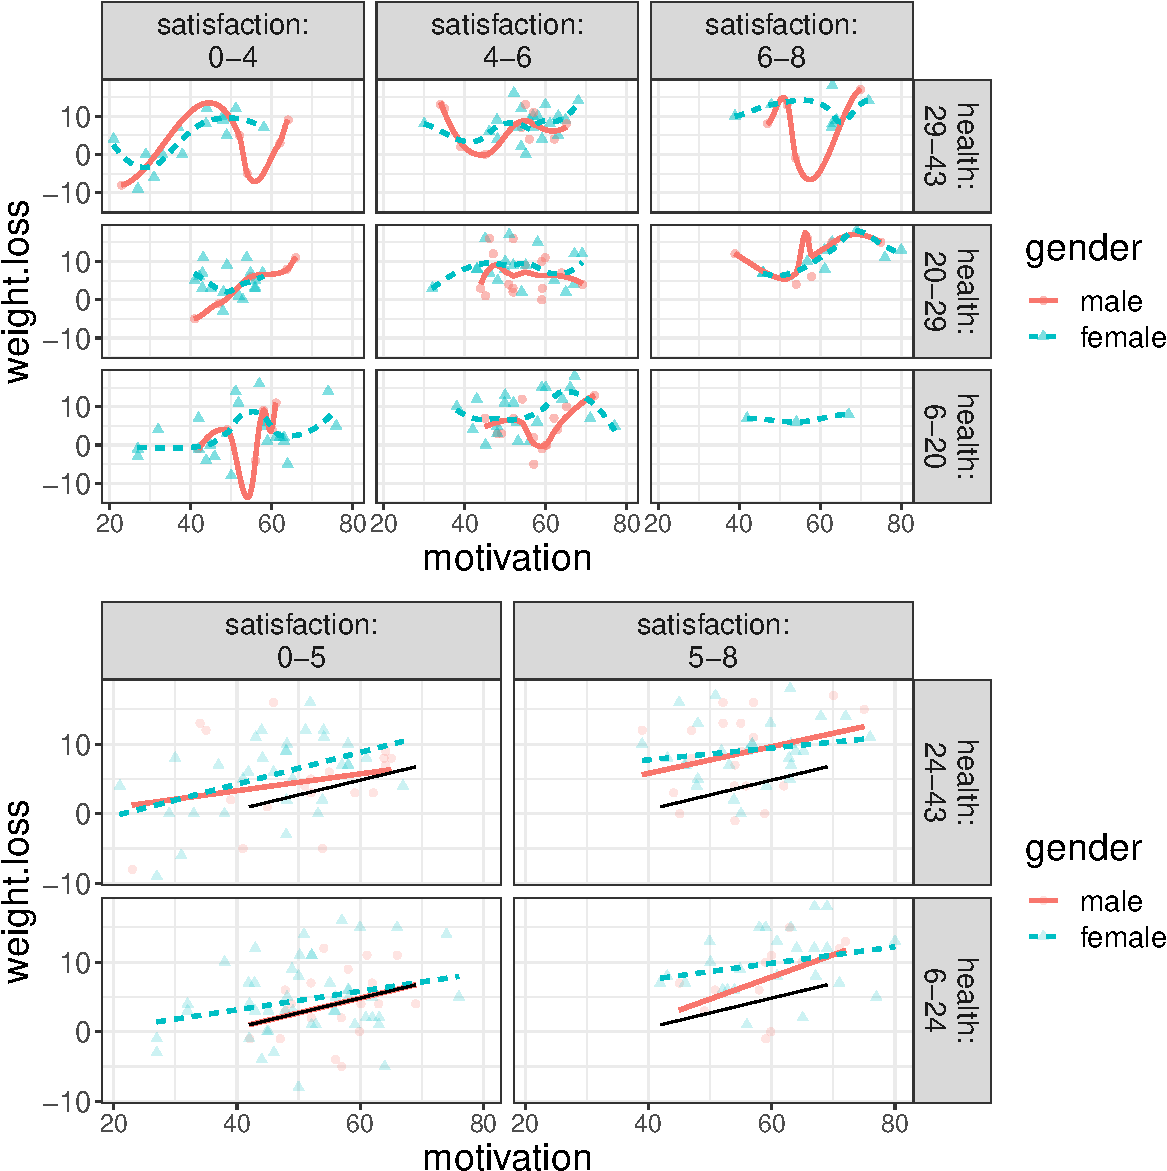
\includegraphics{flexplot_manual_files/figure-latex/threeway-1.pdf}
\caption{\label{fig:threeway}Multivariate relationship between five
variables. Each Flexplot slot is occupied and it's difficult to
interpret what is going on in the top figure, though the use of
regression lines instead of loess lines, removing standard errors,
reducing transparency of the datapoints, adding ghost lines, and
reducing the number of bins have made it easier to interpret (bottom
image).}
\end{figure}

\chapter*{Combining Modeling and
Visualizations}\label{combining-modeling-and-visualizations}
\addcontentsline{toc}{chapter}{Combining Modeling and Visualizations}

Visualization is great for conveying general trends and patterns.
However, it can be difficult to make decisions based on graphics,
particularly when the pattern isn't striking. For example, in Figure
@ref(fig:threeway\}, I don't feel entirely comfortable rejecting the
idea that there are no interactions present in the model. Statistics, on
the other hand, put visual patterns into concrete numbers that assist
with statistical decision-making. Furthermore, it is easy to engage in
confirmation bias when viewing a graphic. Statistics provide a
much-needed reality check. As such, the two, statistics and
visualizations, ought to proceed hand in hand. Fortunately, Flexplot was
designed to compliment statistical analysis (and vice versa). More
specifically, Flexplot has two additional visualization functions, as
well as two functions dedicated to statistical analysis.

\section*{Visualize Function}\label{visualize-function}
\addcontentsline{toc}{section}{Visualize Function}

As I've mentioned repeatedly, one of the primary purposes of Flexplot is
provide visualization for statistical models. The \texttt{visualize()}
function is designed to do exactly that. Much like \texttt{summary()},
or \texttt{coef()}, \texttt{visualize()} is an R method within Flexplot
that can be applied to diverse sorts of models, including \texttt{lmer},
\texttt{lm}, and \texttt{glm}. What \texttt{visualize()} does is attempt
to generate a graphic that matches the formula used in a fitted model.
Not only will \texttt{visualize()} plot a graphic to match the analysis,
but it will also show diagnostic plots. For example, if we were to fit
an ANCOVA model, we could visualize it as follows:

\begin{Shaded}
\begin{Highlighting}[]
\NormalTok{model =}\StringTok{ }\KeywordTok{lm}\NormalTok{(weight.loss}\OperatorTok{~}\NormalTok{motivation}\OperatorTok{+}\NormalTok{therapy.type, }
           \DataTypeTok{data=}\NormalTok{exercise_data)}
\KeywordTok{visualize}\NormalTok{(model)}
\end{Highlighting}
\end{Shaded}

For multivariate data, visualize will default to producing two graphics
to match the analysis: one AVP (top right graphics in Figure
@ref(fig:ancova\}) and one other plot that will use panels and/or
colors/symbols/lines. It will also generate diagnostic plots (histogram
of the residuals, residual dependence plots, and S-L plots). The user
can specify \emph{just} a plot of the model
(\texttt{visualize(model1,\ "model")}), or \emph{just} a plot of the
diagnostics (\texttt{visualize(model1,\ "residuals")}). Additionally,
visualize can take \texttt{flexplot()} arguments and even a
\texttt{flexplot()} formula, as demonstrated in Figure
@ref(fig:ancova2\}

\begin{Shaded}
\begin{Highlighting}[]
\NormalTok{model =}\StringTok{ }\KeywordTok{lm}\NormalTok{(weight.loss}\OperatorTok{~}\NormalTok{motivation}\OperatorTok{+}\NormalTok{therapy.type, }\DataTypeTok{data=}\NormalTok{exercise_data)}
\KeywordTok{visualize}\NormalTok{(model, }\DataTypeTok{formula =}\NormalTok{ weight.loss}\OperatorTok{~}\NormalTok{motivation}\OperatorTok{|}\NormalTok{therapy.type, }
          \DataTypeTok{ghost.line=}\StringTok{"red"}\NormalTok{, }\DataTypeTok{se=}\NormalTok{F, }\DataTypeTok{method=}\StringTok{"lm"}\NormalTok{)}
\end{Highlighting}
\end{Shaded}

Figure \ref{fig:mixed} shows the \texttt{visualize()} function for a
mixed model. With mixed models, \texttt{visualize()} randomly samples
from the random effects (\texttt{Subject} in this case) and plots that
as a variable in the graphic, and its location on the graph depends on
whether the user specifies \texttt{formula}. If they do not,
\texttt{visualize()} will default to placing it in the second slot. This
allows the user to visualize a subset of the subjects in a mixed model
to ensure the model chosen is appropriate.

\begin{Shaded}
\begin{Highlighting}[]
\KeywordTok{require}\NormalTok{(lme4)}
\KeywordTok{data}\NormalTok{(math)}
\NormalTok{model =}\StringTok{ }\KeywordTok{lmer}\NormalTok{(MathAch}\OperatorTok{~}\NormalTok{Sex }\OperatorTok{+}\StringTok{ }\NormalTok{SES }\OperatorTok{+}\StringTok{ }\NormalTok{(SES}\OperatorTok{|}\NormalTok{School), }\DataTypeTok{data=}\NormalTok{math)}
\KeywordTok{visualize}\NormalTok{(model, }
  \DataTypeTok{formula =}\NormalTok{ MathAch}\OperatorTok{~}\StringTok{ }\NormalTok{Sex }\OperatorTok{+}\StringTok{ }\NormalTok{School}\OperatorTok{|}\StringTok{ }\NormalTok{SES, }
  \DataTypeTok{sample=}\DecValTok{30}\NormalTok{)}
\end{Highlighting}
\end{Shaded}

\section*{\texorpdfstring{\texttt{compare.fits()}
Function}{compare.fits() Function}}\label{compare.fits-function}
\addcontentsline{toc}{section}{\texttt{compare.fits()} Function}

Another function in Flexplot is the \texttt{compare.fits()} function.
Very often in statistical modeling, we are interested in comparing two
models, such as one with and one without an interaction term. There are
many statistics available that allow easy comparison between models,
such as the AIC, BIC, Bayes Factor, \(R^2\), p-values, etc. However, it
is again important to \emph{see} how the two models differ in terms of
fit. On multiple occasions, I have found various statistics show
preference for one model, yet the visuals show the two models differ in
only trivial ways.

That's where \texttt{compare.fits()} comes in. It is simply a wrapper
for the \texttt{predict()} function, combined with the graphing
capabilities of Flexplot. More specifically, \texttt{compare.fits()}
will overlay the fit of both models onto the raw data. For example,
Figure \ref{fig:compare} shows the fit of two different models, one that
includes an interaction and the other that does not. The arguments are
very similar to \texttt{flexplot()}, but with the addition of the model
objects. Likewise, \texttt{compare.fits()} takes many of the same
arguments. In this example, I've overlaid a black ghost line. Notice
that the two lines (from \texttt{lm} and \texttt{interaction}) generate
very similar predictions across the range of data, suggesting that a
main effects model may be sufficient.

\begin{Shaded}
\begin{Highlighting}[]
\NormalTok{model.me =}\StringTok{ }\KeywordTok{lm}\NormalTok{(weight.loss}\OperatorTok{~}\NormalTok{motivation}\OperatorTok{+}\NormalTok{therapy.type, }\DataTypeTok{data=}\NormalTok{exercise_data)}
\NormalTok{model.int =}\StringTok{ }\KeywordTok{lm}\NormalTok{(weight.loss}\OperatorTok{~}\NormalTok{motivation}\OperatorTok{*}\NormalTok{therapy.type, }\DataTypeTok{data=}\NormalTok{exercise_data)}
\KeywordTok{compare.fits}\NormalTok{(weight.loss}\OperatorTok{~}\NormalTok{motivation }\OperatorTok{|}\StringTok{ }\NormalTok{therapy.type, }
             \DataTypeTok{data=}\NormalTok{exercise_data, model.me, model.int, }\DataTypeTok{ghost.line=}\StringTok{"black"}\NormalTok{)}\OperatorTok{+}
\StringTok{      }\NormalTok{ggplot2}\OperatorTok{::}\KeywordTok{facet_grid}\NormalTok{(}\OperatorTok{~}\NormalTok{therapy.type, }
                          \DataTypeTok{labeller =}\NormalTok{ ggplot2}\OperatorTok{::}\KeywordTok{labeller}\NormalTok{(}\DataTypeTok{therapy.type=}\NormalTok{label_value))}
\end{Highlighting}
\end{Shaded}

\chapter*{Functions Devoted to
Estimation}\label{functions-devoted-to-estimation}
\addcontentsline{toc}{chapter}{Functions Devoted to Estimation}

The Flexplot package specializes in visualization, providing easy-to-use
tools for graphical data analysis. However, it also has a small
collection of non-visual functions that can be used hand-in hand with
visuals. These functions include the \texttt{estimates()} method and
\texttt{model.comparison()}.

\section*{The estimates() function}\label{the-estimates-function}
\addcontentsline{toc}{section}{The estimates() function}

The \texttt{estimates()} function was designed to report paremeter
estimates and estimates of effect size. Much like \texttt{flexplot()},
many of the decisions are made in the background. And like
\texttt{visualize()}, \texttt{estimates()} takes a fitted object as
input. \texttt{estimates()} will then determine which estimates are most
appropriate. For grouping variables, \texttt{estimates()} will report
means, mean differences, and cohen's \(d\), as well as 95\% confidence
intervals. For numeric variables, \texttt{estimates()} will report the
intercept, slopes, and standardized slopes, also with corresponding
confidence intervals. Additionally, it will report the model \(R^2\), as
well as the semi-partial \(R^2\) associated with each effect in the
model, except when there are interactions in the model. (With
interactions present, it doesn't make sense to interpret main effects,
which is why \texttt{estimates()} only reports the semi-partial for the
interaction effect).

\begin{Shaded}
\begin{Highlighting}[]
\KeywordTok{estimates}\NormalTok{(model.int)}
\end{Highlighting}
\end{Shaded}

\begin{verbatim}
## Model R squared:
## 0.222 (0.12, 0.32)
## 
## Semi-Partial R squared:
## motivation:therapy.type 
##                   0.006 
## Correlation:
##  NA 
## 
## Estimates for Factors:
##      variables  levels estimate lower upper
## 1 therapy.type control     4.09  2.81  5.38
## 2                  beh     7.86  6.74  8.99
## 3                  cog     7.74  6.46  9.02
## 
## 
## Mean Differences:
##      variables  comparison difference lower upper cohens.d
## 1 therapy.type beh-control       3.77  0.71  6.84     0.75
## 2         <NA> cog-control       3.65  0.77  6.54     0.72
## 3         <NA>     cog-beh      -0.12 -2.99  2.75    -0.02
## 
## 
## Estimates for Numeric Variables = 
##     variables estimate  lower upper std.estimate std.lower std.upper
## 1 (Intercept)    -5.77 -11.84  0.31         0.00      0.00      0.00
## 2  motivation     0.18   0.07  0.29         0.35     -0.33      1.03
\end{verbatim}

The estimates shown support the conclusions gleaned from Figure
@ref(fig:ancova\}, namely that the addition of the interaction likely
isn't improving the fit enough to consider keeping.

\section*{\texorpdfstring{The \texttt{model.comparison()}
function}{The model.comparison() function}}\label{the-model.comparison-function}
\addcontentsline{toc}{section}{The \texttt{model.comparison()} function}

The final function I will mention is the \texttt{model.comparison()}
function. This is similar to the \texttt{anova()} function in base R,
but it includes additional estimates, including AIC, BIC, and the
BIC-derived Bayes Factor. Additionally, \texttt{model.comparison()}
works on both nested and non-nested functions. When used on non-nested
functions, it will compute AIC, BIC, and Bayes Factor. Also, the
\texttt{model.comparison()} function will report the quantiles of the
\emph{differences} in prediction, in standardized units. The
\texttt{model.comparison()} below compares the main effects and the
interaction model. The last reported numbers indicate that the maximum
difference in prediction between the two models is only about a third of
a standard deviation, while the median difference is only about 0.05
standard deviations, suggesting the predictions are quite similar. Also,
all statistics (AIC, BIC, Bayes Factor, p-value, and probably \(R^2\))
support the more simplified main effects model.

\begin{Shaded}
\begin{Highlighting}[]
\KeywordTok{model.comparison}\NormalTok{(model.int, model.me)}
\end{Highlighting}
\end{Shaded}

\begin{verbatim}
## $statistics
##                aic      bic bayes.factor   p.value r.squared
## model.int 1223.041 1246.129   0.01049379 0.4871878 0.2222871
## model.me  1220.523 1237.015  95.29443074        NA 0.2165001
## 
## $pred.difference
##           0%          25%          50%          75%         100% 
## 0.0005508775 0.0172347143 0.0499237628 0.0783236513 0.3483202575
\end{verbatim}

\chapter*{Concluding Thoughts}\label{concluding-thoughts}
\addcontentsline{toc}{chapter}{Concluding Thoughts}

In summary, this paper has sought to demonstrate the utility of the
Flexplot package. This visual approach to data analysis has many
advantages, including emphasizing uncertainty, improving encoding, and
increasing communication with lay audiences. The simplified
formula-based grammar of graphics makes many basic and advanced plotting
functions much easier to produce, and does so using
scientifically-derived principals of human perception. Additionally,
Flexplot allows tools that permit seamless integration of statistical
analysis with visual interpretation.

\chapter*{}\label{section}
\addcontentsline{toc}{chapter}{}

\hypertarget{refs}{}
\hypertarget{ref-Baker2016a}{}
Baker, Monya. 2016. ``1,500 Scientists Lift the Lid on
Reproducibility.'' \emph{Nature} 533 (7604): 452--54.
doi:\href{https://doi.org/10.1038/533452a}{10.1038/533452a}.

\hypertarget{ref-Cleveland1994}{}
Cleveland, William S. 1994. ``Coplots, nonparametric regression, and
conditionally parametric fits.'' \emph{Lecture Notes-Monograph Series}.
JSTOR, 21--36.

\hypertarget{ref-Correll2015a}{}
Correll, Michael A. 2015. ``Improving Visual Statistics.''

\hypertarget{ref-Fife2019}{}
Fife, Dustin A. 2019. ``Glinmod {[}Computer Software{]}.''

\hypertarget{ref-Nelson2018}{}
Nelson, Leif D., Joseph P. Simmons, and Uri Simonsohn. 2018.
``Psychology's Renaissance.'' \emph{Annu. Rev. Psychol} 69: 511--45.
doi:\href{https://doi.org/10.1146/annurev-psych-122216}{10.1146/annurev-psych-122216}.

\hypertarget{ref-Nosek2018}{}
Nosek, Brian A., Charles R. Ebersole, Alexander C. DeHaven, and David T.
Mellor. 2018. ``The preregistration revolution.'' \emph{Proceedings of
the National Academy of Sciences}.
doi:\href{https://doi.org/10.1073/pnas.1708274114}{10.1073/pnas.1708274114}.

\hypertarget{ref-OpenScienceCollaboration2015}{}
Open Science Collaboration. 2015. ``Estimating the reproducibilty of
psychological science.'' \emph{Science}.
doi:\href{https://doi.org/10.1126/science.aac4716}{10.1126/science.aac4716}.

\hypertarget{ref-Padilla2015}{}
Padilla, Lace M., Grace Hansen, Ian T. Ruginski, Heidi S. Kramer,
William B. Thompson, and Sarah H. Creem-Regehr. 2015. ``The influence of
different graphical displays on nonexpert decision making under
uncertainty.'' \emph{Journal of Experimental Psychology: Applied} 21
(1): 37--46.
doi:\href{https://doi.org/10.1037/xap0000037}{10.1037/xap0000037}.

\hypertarget{ref-Pashler2012a}{}
Pashler, Harold, and Eric-Jan Wagenmakers. 2012. ``Editors' Introduction
to the Special Section on Replicability in Psychological Science.''
\emph{Perspectives on Psychological Science} 7 (6). SAGE
PublicationsSage CA: Los Angeles, CA: 528--30.
doi:\href{https://doi.org/10.1177/1745691612465253}{10.1177/1745691612465253}.

\hypertarget{ref-Tay2016}{}
Tay, Louis, Scott Parrigon, Qiming Huang, and James M. LeBreton. 2016.
``Graphical Descriptives.'' \emph{Perspectives on Psychological
Science}.

\hypertarget{ref-Tukey1990}{}
Tukey, John W., and P A Tukey. 1990. ``Strips Displaying Empirical
Distributions: I. Textured Dot Strips.'' Bellcore.

\hypertarget{ref-Wickham2010}{}
Wickham, Hadley. 2010. ``A Layered Grammar of Graphics.''
doi:\href{https://doi.org/10.1198/jcgs.2009.07098}{10.1198/jcgs.2009.07098}.

\hypertarget{ref-Wilkinson1999}{}
Wilkinson, Leland. 1999. ``Statistical methods in psychology journals:
Guidelines and explanations.'' \emph{American Psychologist} 54 (8):
594--604.
doi:\href{https://doi.org/10.1037/0003-066X.54.8.594}{10.1037/0003-066X.54.8.594}.


\end{document}
